\documentclass{beamer}
\usepackage{beamerthemesplit}
\setbeamertemplate{footline}[number frame]
\usetheme{Darmstadt}%CopenhagenMadridJuanLesPins
%\setbeamercolor{structure}{fg=green!60!blue}
\usepackage{graphicx,euscript}
%\usepackage[dvips]{graphicx}
\usepackage[T1]{fontenc}
\usepackage{hyphenat}
\usepackage{stmaryrd}
\usepackage{color}
\usepackage{caption}
\usepackage{marvosym}
\usepackage[latin1]{inputenc}
\usepackage{amsmath}
\usepackage{mathcomp}
%\usepackage{graphics}
\usepackage{subfigure}
\usepackage{dsfont}
\usepackage{epsfig}
\usepackage{amssymb}
\usepackage{epstopdf}
\usepackage[curves]{struktex}
\usepackage[ruled]{algorithm}
\usepackage{algorithmic}

\DeclareMathOperator*{\argmin}{\arg\!\min}

\beamertemplatenavigationsymbolsempty
\title[Nonlinear Model Order Reduction for Optimal Control]{\bf Nonlinear Model Order Reduction for Optimal Control of Burgers' Equation}
\titlegraphic{
\includegraphics[scale=0.09]{TU_Delft_logo1.png} \hspace{1cm}
   
\includegraphics[scale=0.5]{cosse_logo.jpg}}
\subtitle{- \textsc{Master thesis} -}
\author{Manuel M. Baumann}
\date{July 15, 2013}
\begin{document}

\frame{
\titlepage
}

\frame{
\frametitle{Table of Contents}
\tableofcontents
}

\section[Introduction]{What is Model Order Reduction (MOR) ?}
\subsection*{}
\frame{
\frametitle{Nonlinear dynamical systems}
Consider the nonlinear dynamical system
\begin{equation}
\begin{split}
\label{nonlinSys}
\dot{\mathbf{y}}(t) &= A \mathbf{y}(t) + \mathbf{F}(t,\mathbf{y}(t)), \quad \mathbf{y}(t) \in \mathbb{R}^{\color{blue} N \color{black}}\\
\mathbf{y}(0) &= \mathbf{y}_0
\end{split}
\end{equation}
\setbeamercovered{transparent}
\begin{itemize}
  \uncover<2->{\item arises in many applications, e.g. mechanical systems, fluid dynamics, neuron modeling, ...}
  \uncover<3->{\item the matrix $A$ represents the linear dynamical behavior and the function $\mathbf{F}$ represents nonlinear dynamics}
  \uncover<4->{\item often \color{blue} large \color{black} dimension of \eqref{nonlinSys} leads to \textit{huge} computational work}
\end{itemize}
}
\frame{
\frametitle{The idea of model order reduction}
Approximate the state via
\begin{align*}
\mathbf{y}(t) \approx U_\ell \tilde{\mathbf{y}}(t), \quad U_\ell \in \mathbb{R}^{N \times \color{blue} \ell \color{black}}, \tilde{\mathbf{y}} \in \mathbb{R}^{\color{blue} \ell \color{black}},
\end{align*}
where the matrix $U_\ell$ consists of orthonormal columns, the so-called \textit{principal components} of $\mathbf{y}$, and \color{blue}$\ell \ll N$\color{black}.\\
\vspace{0.7cm}
\color{red}Galerkin projection \color{black} of the original full-order system leads to a reduced $\ell \times \ell$ system of equations:
\begin{align*}
&U_\ell^T (U_\ell \dot{\tilde{\mathbf{y}}} - A U_\ell \tilde{\mathbf{y}} - \mathbf{F}(t,U_\ell \tilde{\mathbf{y}})) = 0 \\ &\Rightarrow \quad \dot{\tilde{\mathbf{y}}} = \underbrace{U_\ell^T A U_\ell}_{=:\tilde{A}}\tilde{\mathbf{y}} +  U_\ell^T \mathbf{F}(t,U_\ell\tilde{\mathbf{y}})
\end{align*}
}
\frame{
\frametitle{Two questions are left...}
Considering the reduced model
\begin{align*}
\dot{\tilde{\mathbf{y}}}(t) = \tilde{A} \tilde{\mathbf{y}}(t) + U_\ell^T \mathbf{F}(t,U_\ell\tilde{\mathbf{y}}(t))
\end{align*}
two questions are left:\\
\hspace{0.4cm}
\setbeamercovered{transparent}
\begin{enumerate}
  \uncover<2->{\item How to obtain the matrix $U_\ell$ of principal components ?}
  \uncover<3->{\item Note that $U_\ell \tilde{\mathbf{y}}(t) \in \mathbb{R}^{\color{blue} N \color{black}}$ is still \color{blue} large\color{black}. How do we evaluate $\mathbf{F}(t,U_\ell\tilde{\mathbf{y}}(t))$ efficiently ?}
\end{enumerate}
}
\section[POD-DEIM algorithm]{The POD-DEIM method}
\subsection{Proper Orthogonal Decomposition (POD)}
\frame{
\frametitle{The Proper Orthogonal Decomposition (POD)}
During the numerical simulation, build up the matrix
\begin{align*}
Y := [\mathbf{y}(t_1),...,\mathbf{y}(t_{n_s})] \in \mathbb{R}^{N \times \color{red} n_s \color{black}},
\end{align*}
with $n_s$ being the \color{red} number of snapshots\color{black}.\\
\vspace{0.5cm}
Perform a Singular Value Decomposition (SVD)
\begin{align*}
Y = U \Sigma V^T
\end{align*}
and let $U_\ell := \texttt{U(:,1:\color{blue}l\color{black})}$ consist of those left singular vectors of $Y$ that correspond to the \color{blue} $\ell$ largest singular values \color{black} in $\Sigma$.
}
\subsection{Discrete Empirical Interpolation Method (DEIM)}
\frame{
\frametitle{The Discrete Empirical Interpolation Method (DEIM)}
Consider the nonlinearity
\begin{align*}
\mathbf{N} := \underbrace{U_\ell^T}_{\ell \times \color{blue}N\color{black}} \underbrace{\mathbf{F}(t,U_\ell\tilde{\mathbf{y}}(t))}_{\color{blue}N\color{black} \times 1}
\end{align*}
The approximation
\begin{align*}
\mathbf{F} \approx W \mathbf{c}, \quad W \in \mathbb{R}^{N \times \color{red}m\color{black}}, \mathbf{c} \in \mathbb{R}^{\color{red}m\color{black}}
\end{align*}
is over determined. Therefore, find projection $\mathcal{P}$ such that:
\begin{align*}
\mathcal{P}^T \mathbf{F} = (\mathcal{P}^T W)\mathbf{c} \quad &\Rightarrow \quad \mathbf{F} \approx W \mathbf{c} = W (\mathcal{P}^T W)^{-1} \mathcal{P}^T \mathbf{F} \\
\quad &\Rightarrow \quad \mathbf{N} \approx U_\ell^T W \underbrace{(\mathcal{P}^T W)}_{\color{red}m\color{black} \times \color{red}m\color{black}}^{-1} \mathcal{P}^T \mathbf{F}(t,U_\ell \mathbf{\tilde y}(t))
\end{align*}
}
\frame{
\frametitle{The Discrete Empirical Interpolation Method (DEIM)}
Consider the nonlinearity
\begin{align*}
\mathbf{N} := \underbrace{U_\ell^T}_{\ell \times \color{blue}N\color{black}} \underbrace{\mathbf{F}(t,U_\ell\tilde{\mathbf{y}}(t))}_{\color{blue}N\color{black} \times 1}
\end{align*}
The approximation
\begin{align*}
\mathbf{F} \approx W \mathbf{c}, \quad W \in \mathbb{R}^{N \times \color{red}m\color{black}}, \mathbf{c} \in \mathbb{R}^{\color{red}m\color{black}}
\end{align*}
is over determined. Therefore, find projection $\mathcal{P}$ such that:
\begin{align*}
\mathcal{P}^T \mathbf{F} = (\mathcal{P}^T W)\mathbf{c} \quad &\Rightarrow \quad \mathbf{F} \approx W \mathbf{c} = W (\mathcal{P}^T W)^{-1} \mathcal{P}^T \mathbf{F} \\
\quad &\Rightarrow \quad \mathbf{N} \approx U_\ell^T W \underbrace{(\mathcal{P}^T W)}_{\color{red}m\color{black} \times \color{red}m\color{black}}^{-1} \color{green} \mathcal{P}^T \mathbf{F}(t,U_\ell \mathbf{\tilde y}(t))\color{black}
\end{align*}
}
\frame{
\begin{algorithm}[H]
\caption{The DEIM algorithm \cite{DEIM}}
\label{alg:DEIM}
\begin{algorithmic}[1]
\STATE \textbf{INPUT: } $\{\mathbf{w}_i\}_{i=1}^m \subset \mathbb{R}^N$  linear independent
\STATE \textbf{OUTPUT: } $\vec \wp = [\wp_1,...,\wp_m]^T \in \mathbb{R}^m, \ \mathcal{P} \in \mathbb{R}^{N \times m}$
\STATE $[|\rho|,\color{red}\wp_1\color{black}] = \max \{|\mathbf{w}_1|\}$
\STATE $W = [\mathbf{w}_1], \color{red}\mathcal{P} = [\mathbf{e}_{\wp_1}]\color{black}, \vec \wp = [\wp_1]$
\FOR{$i = 2$ to $m$}
\STATE Solve $(\mathcal{P}^T W) \mathbf{c} = \mathcal{P}^T \mathbf{w}_i$ for $\mathbf{c}$
\STATE $\mathbf{r} = \mathbf{w}_i - W \mathbf{c}$
\STATE $[|\rho|,\color{red}\wp_i\color{black}] = \max \{|\mathbf{r}|\}$
\STATE $W \leftarrow [W \ \mathbf{w}_i], \color{red} \mathcal{P} \leftarrow [\mathcal{P} \ \mathbf{e}_{\wp_i}]\color{black}, \vec \wp \leftarrow \begin{bmatrix} \vec \wp \\ \wp_i \end{bmatrix}$
\ENDFOR
\end{algorithmic}
\end{algorithm}
}
\frame{
\frametitle{The product $\mathcal{P}^T \mathbf{F}$ is a selection of entries}
Let $m=3$. Suppose the DEIM-algorithm has chosen indices $\wp_1,...,\wp_m$ such that:
%\begin{align*}
%\mathcal{P}^T \mathbf{F} = \begin{bmatrix} 0 & \hdots & 1 & \hdots & 0\\
%                                           0 & \color{red}1\color{black} & \hdots & \hdots & 0\\
%                                           0 & \hdots & 0 & 1 & 0  \end{bmatrix}
%                                           \begin{bmatrix} F_1\\\color{red}F_2\color{black}\\ \vdots \\ F_N \end{bmatrix} = \begin{bmatrix} F_{\wp_1}\\\color{red}F_{\wp_2}\color{black}\\F_{\wp_m}\end{bmatrix}
%\end{align*}
%Therefore, $\color{green}\mathcal{P}^T \mathbf{F}\color{black}$ is equal to $[\mathbf{F}_{\wp_1},...,\mathbf{F}_{\wp_m}]^T$.
\begin{figure}[H]
\centering
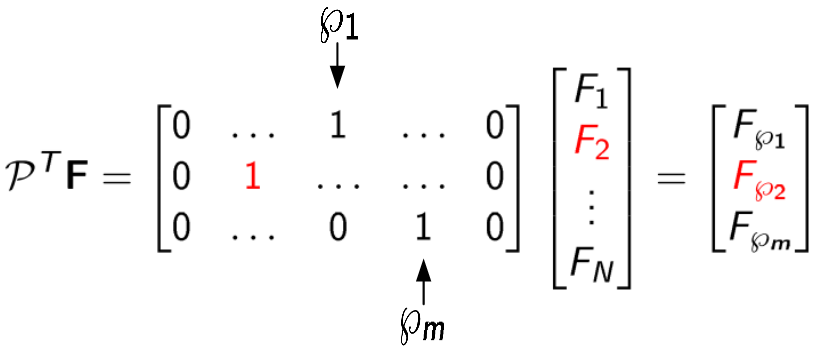
\includegraphics[width=0.7\textwidth]{figures/deimMaVec.png}
\end{figure}
Therefore, suppose $\mathbf{F}(\cdot)$ acts pointwise, we obtain:
\begin{align*}
\mathbf{N} &\approx U_\ell^T W (\mathcal{P}^T W)^{-1} \mathcal{P}^T \mathbf{F}(t,U_\ell \mathbf{\tilde y}(t))\\
&= \underbrace{U_\ell^T W (\mathcal{P}^T W)^{-1}}_{\ell \times m} \underbrace{\mathbf{F}(t,\mathcal{P}^T U_\ell \mathbf{\tilde y}(t))}_{m \times 1}
\end{align*}
}
\subsection{Application: MOR for Burgers' equation}
\frame{
\begin{block}{The nonlinear 1D Burgers' model}
\begin{equation*}
\begin{split}
y_t + \left( \frac{1}{2}y^2 - \nu y_x\right)_x = f&, \quad (x,t) \in (0,L) \times (0,T), \\
y(t,0) = y(t,L) = 0&, \quad t \in (0,T), \\
y(0,x) = y_0(x)&, \quad x \in (0,L).
\end{split}
\end{equation*}
\end{block}
\vspace{0.4cm}
FEM-discretization in space leads to:
\begin{align*}
M \dot{\mathbf{y}}(t) &= -\frac{1}{2} B \mathbf{y}^2(t) - \nu C \mathbf{y}(t) + \mathbf{f}, \quad t > 0 \\
\mathbf{y}(0) &= \mathbf{y}_0
\end{align*}
}
\frame{
\frametitle{POD-DEIM for Burgers' equation}
\scriptsize{
Suppose, $\Phi_\ell$ is an M-orthogonal POD basis.
\begin{block}{The POD reduced Burgers' equation}
\begin{align*}
\overbrace{\Phi_\ell^T M \Phi_\ell}^{=I_\ell}\dot{\mathbf{\tilde y}}(t) &= -\frac{1}{2} \color{red} \Phi_\ell^T B \color{black} (\Phi_{\ell} \mathbf{\tilde y}(t))^2 - \nu \color{blue}\Phi_\ell^T C \Phi_\ell \color{black} \mathbf{\tilde y}(t)\\
\Rightarrow \quad \dot{\mathbf{\tilde y}}(t) &= -\frac{1}{2} \color{red} B_{\ell} \color{black} (\Phi_{\ell} \mathbf{\tilde y}(t))^2 - \nu \color{blue} C_{\ell} \color{black} \mathbf{\tilde y}(t)
\end{align*}
\end{block}
}
\vspace{0.2cm}
\setbeamercovered{transparent}
\uncover<2->{
\scriptsize{
Next, obtain $W$ via a truncated SVD of $[\mathbf{y}^2(t_1),...,\mathbf{y}^2(t_{n_s})]$ and apply DEIM to the columns of $W$.
\begin{block}{The POD-DEIM reduced Burgers' equation}
\begin{align*}
 \dot{\mathbf{\tilde y}}(t) &= -\frac{1}{2} \color{red} \tilde{B} \color{black} (\color{green} \tilde{F} \color{black} \mathbf{\tilde y}(t))^2 - \nu \color{blue} \tilde{C} \color{black} \mathbf{\tilde y}(t),
\end{align*}
with $\color{red} \tilde{B} = \Phi_\ell^T B W (\mathcal{P}^T W)^{-1} \in \mathbb{R}^{\ell \times m} \color{black}$, $\color{green} \tilde{F} = \mathcal{P}^T \Phi_\ell \in \mathbb{R}^{m \times \ell} \color{black}$, and $\color{blue} \tilde{C} = C_\ell \in \mathbb{R}^{\ell \times \ell} \color{black}$.
\end{block}
}}
}
\frame{
\begin{figure}[H]
  \centering
  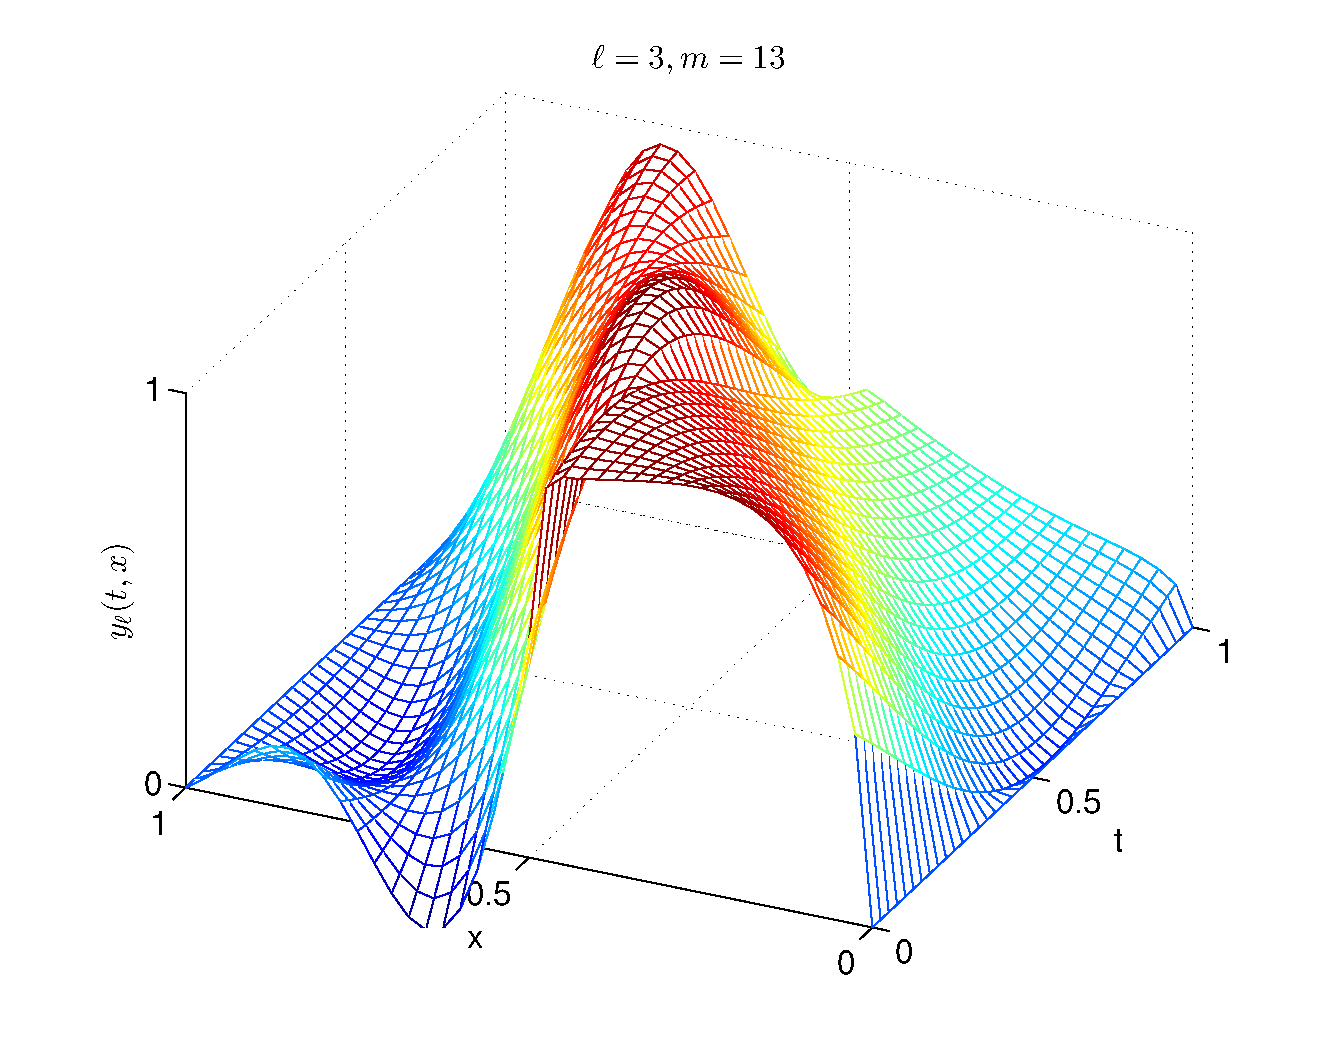
\includegraphics[width=\textwidth]{figures/l3_new.eps}
\end{figure}
}
\frame{
\begin{figure}[H]
  \centering
  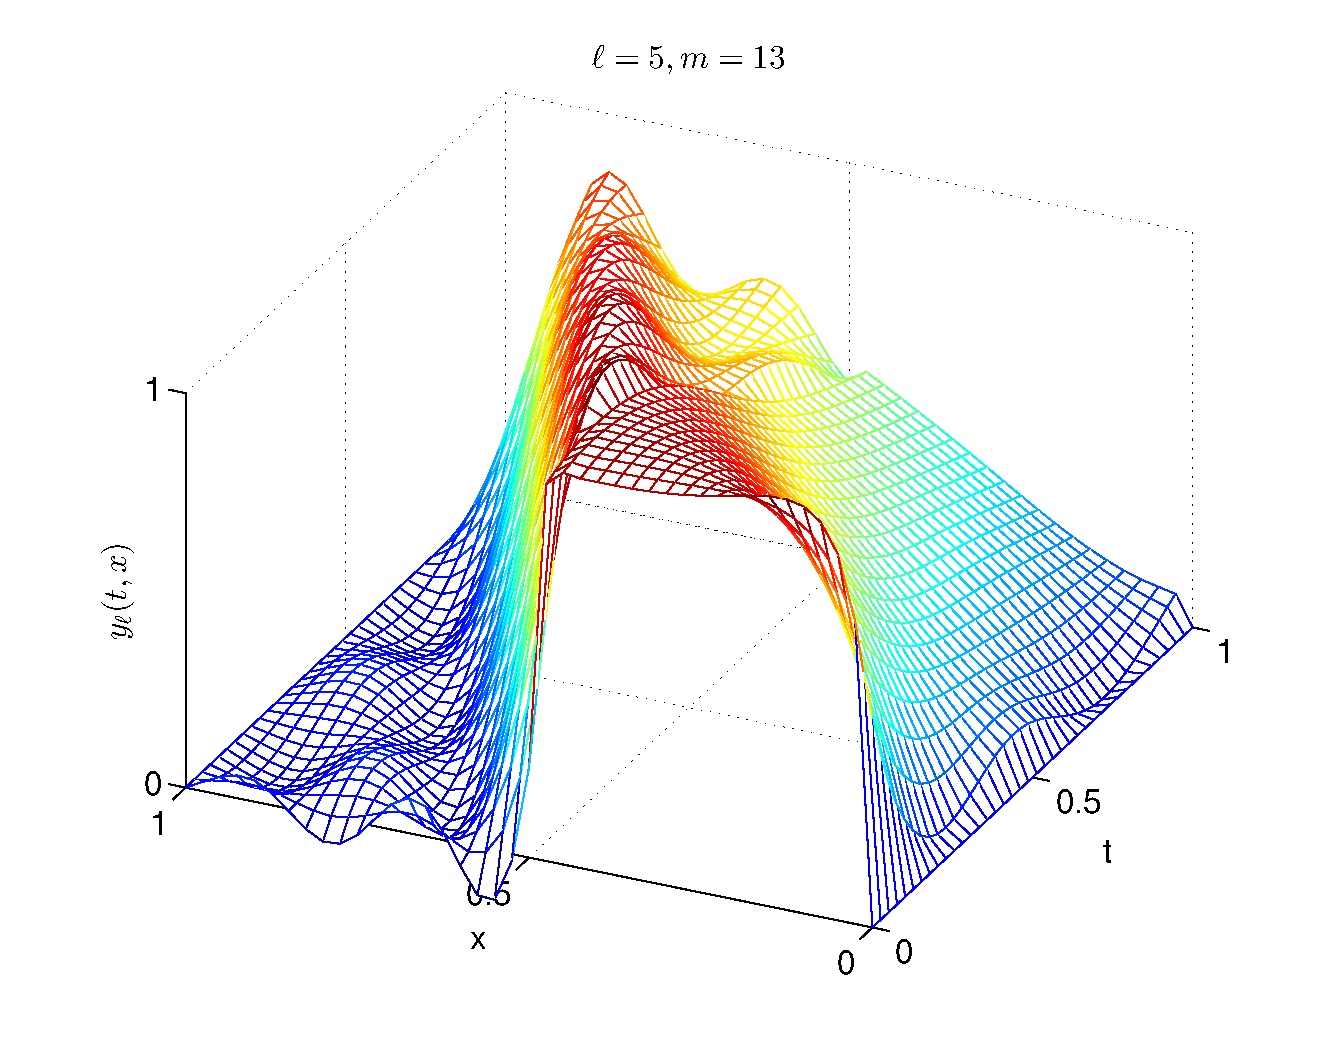
\includegraphics[width=\textwidth]{figures/l5_new.eps}
\end{figure}
}
\frame{
\begin{figure}[H]
  \centering
  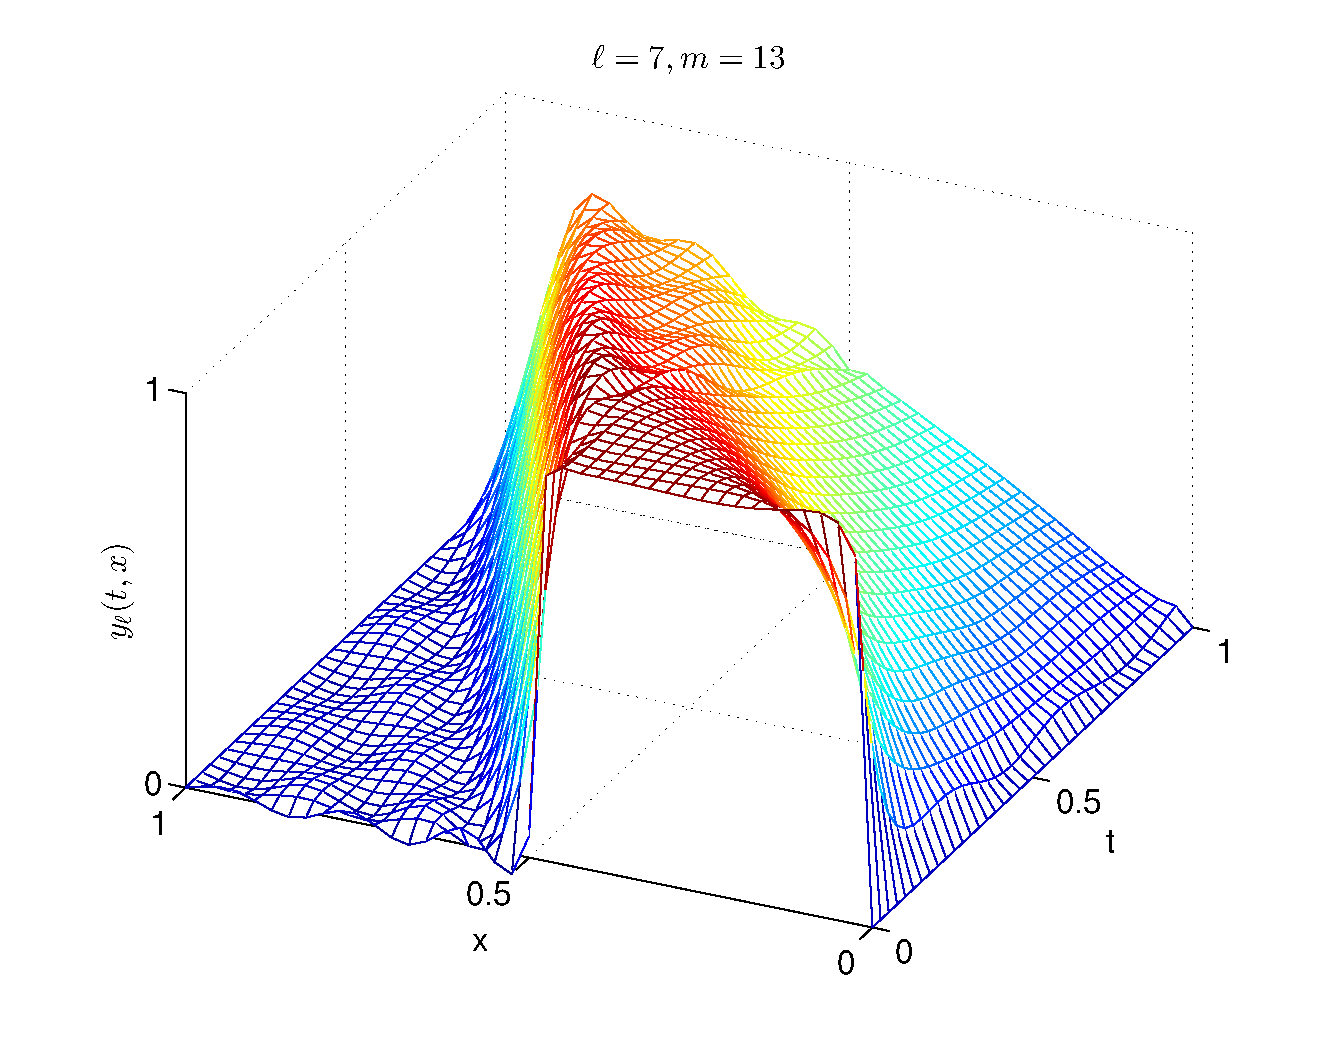
\includegraphics[width=\textwidth]{figures/l7_new.eps}
\end{figure}
}
\frame{
\begin{figure}[H]
  \centering
  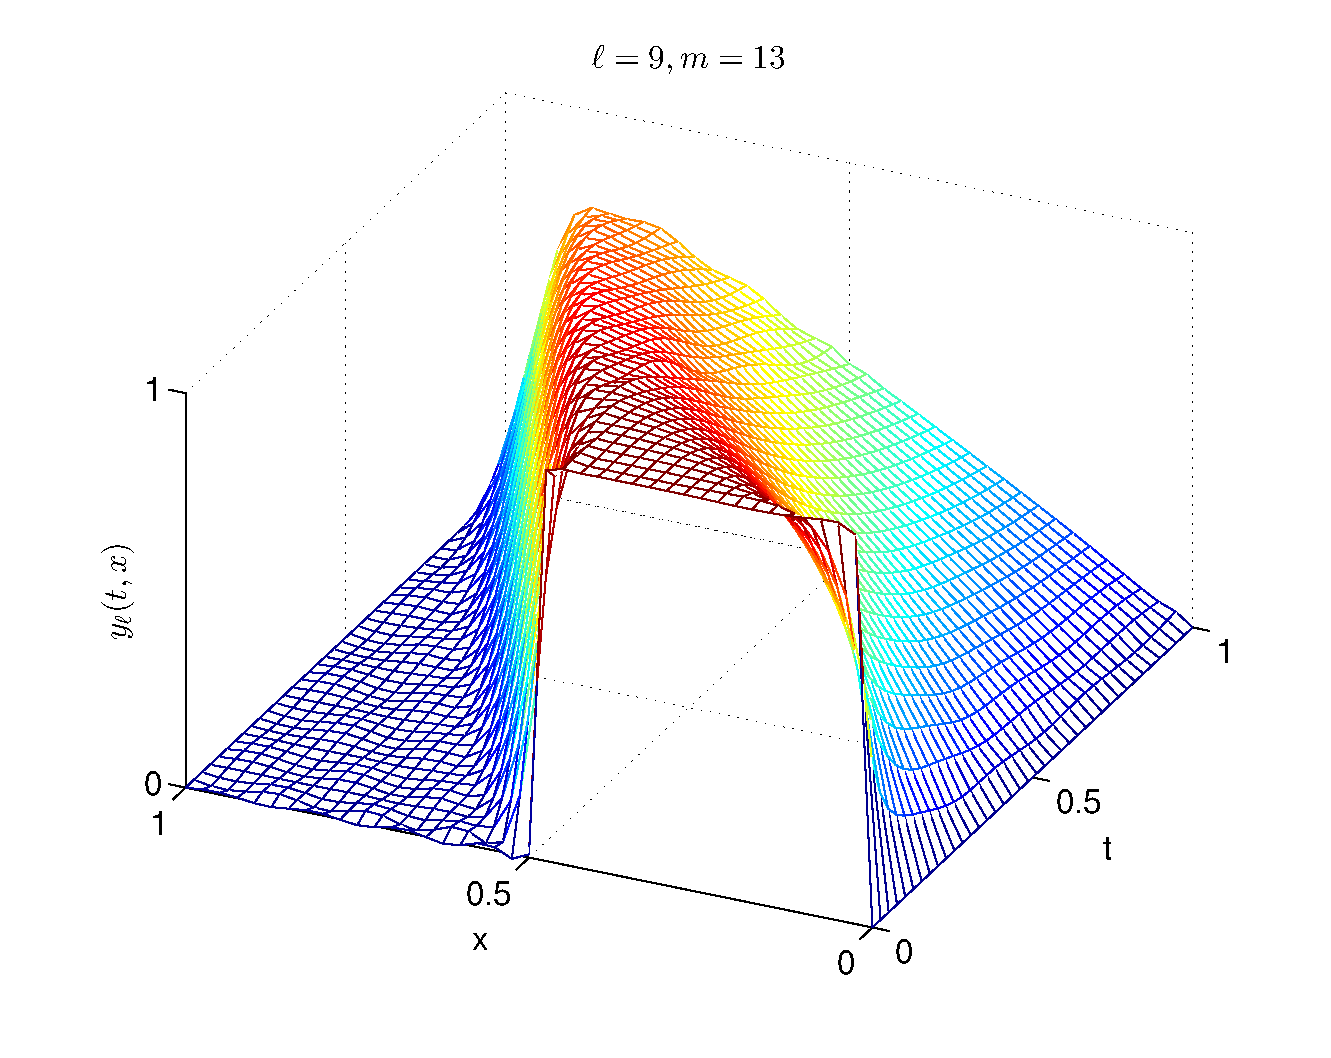
\includegraphics[width=\textwidth]{figures/l9_new.eps}
\end{figure}
}
\frame{
\begin{figure}[H]
  \centering
  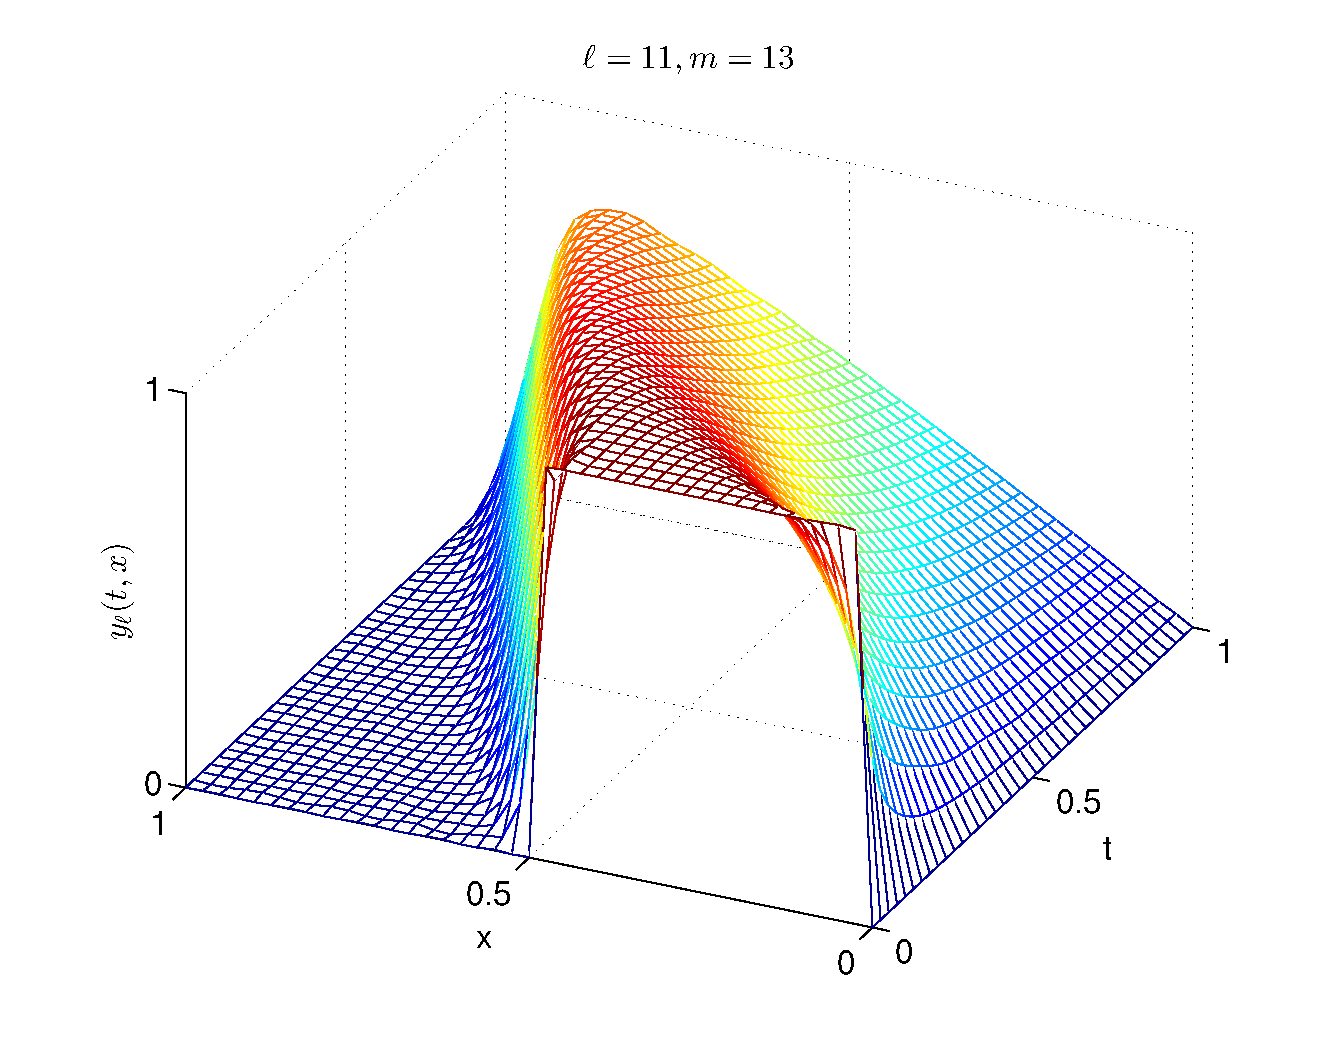
\includegraphics[width=\textwidth]{figures/l11_new.eps}
\end{figure}
}
\frame{
\frametitle{Computational Speedup}
\begin{table}[H]
\tiny
\centering
\begin{tabular}{|c|c|c|c|c|c|c|c|c|c|}
\cline{1-10}
 & \multicolumn{3}{ c| }{$\nu = 0.01$} & \multicolumn{3}{ c| }{$\nu = 0.001$}& \multicolumn{3}{ c| }{$\nu = 0.0001$}\\ \cline{2-10}
 & Full & POD & DEIM & Full & POD & DEIM & Full & POD & DEIM \\ \cline{1-10}
$N$/$\ell$/$m$ & $80$ &$ 11 $&$(11,13)$ & $200$&$35 $& $(35,40)$  & $800$&$40 $& $(40,55)$ \\ \cline{1-10}
$t_{setup}[s]$        & -      &0.003      &0.011       & -    &0.009&0.021 & -& 0.0729&0.182\\ \cline{1-10}
$t_{PDEsol}[s]$   &  0.068     &0.047      &0.040       & 0.232&0.12&0.055 & 4.416&0.276&0.085\\ \cline{1-10}
$\bar{e}[10^{-4}]$   & -      &6.13       &6.46        & -    &6.12&6.85 & -&7.43& 7.66\\ \cline{1-10}
$S_P^{(1)}$           & -      &1.35       &1.34        & -    &1.74&3.03 & -&12.54&16.52\\ \cline{1-10}
$S_P^{(2)}$           & -      &1.44       &1.71        & -    &1.88&4.21 & -&\color{red}15.85\color{black}&\color{red}51.85\color{black}\\ \cline{1-10}
\end{tabular}
\end{table}
\begin{figure}[H]
\centering
%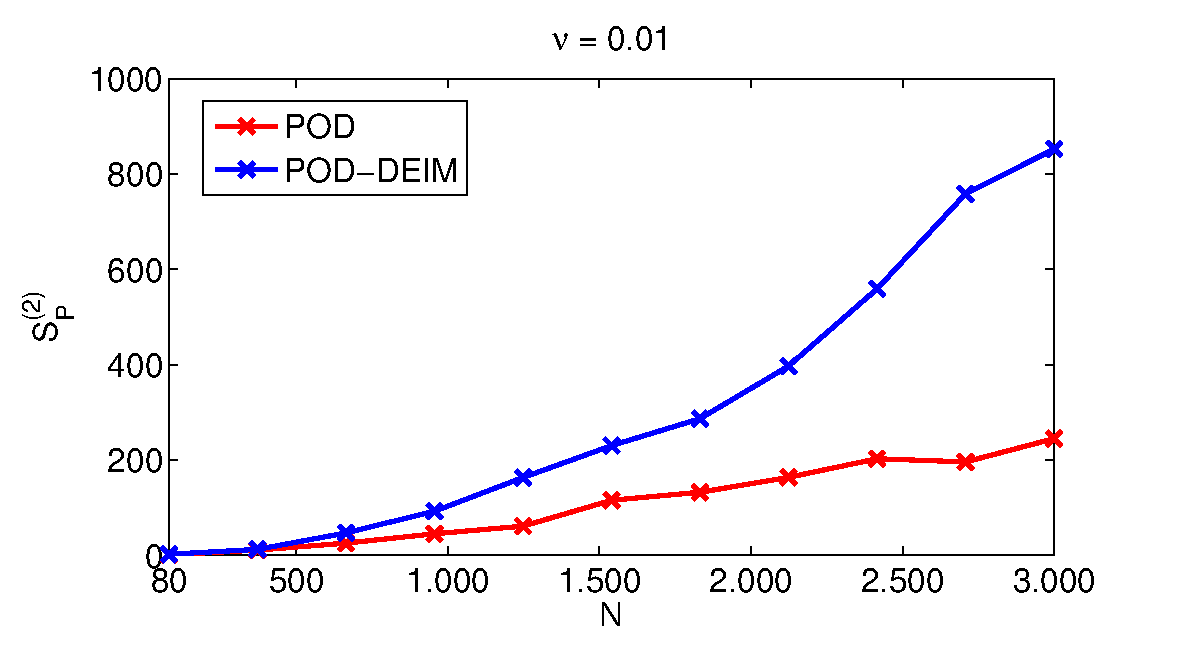
\includegraphics{figures/PODDEIM_Sp2.eps}
\subfigure{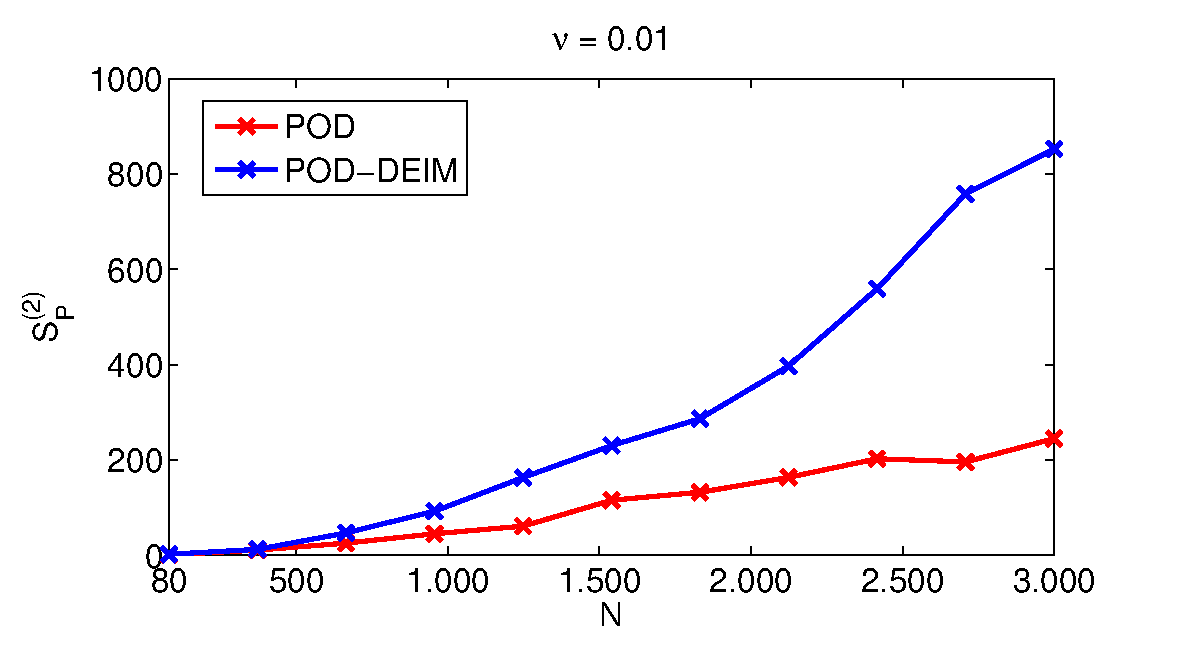
\includegraphics[width=0.49\textwidth]{figures/PODDEIM_Sp2}}\hfill
\subfigure{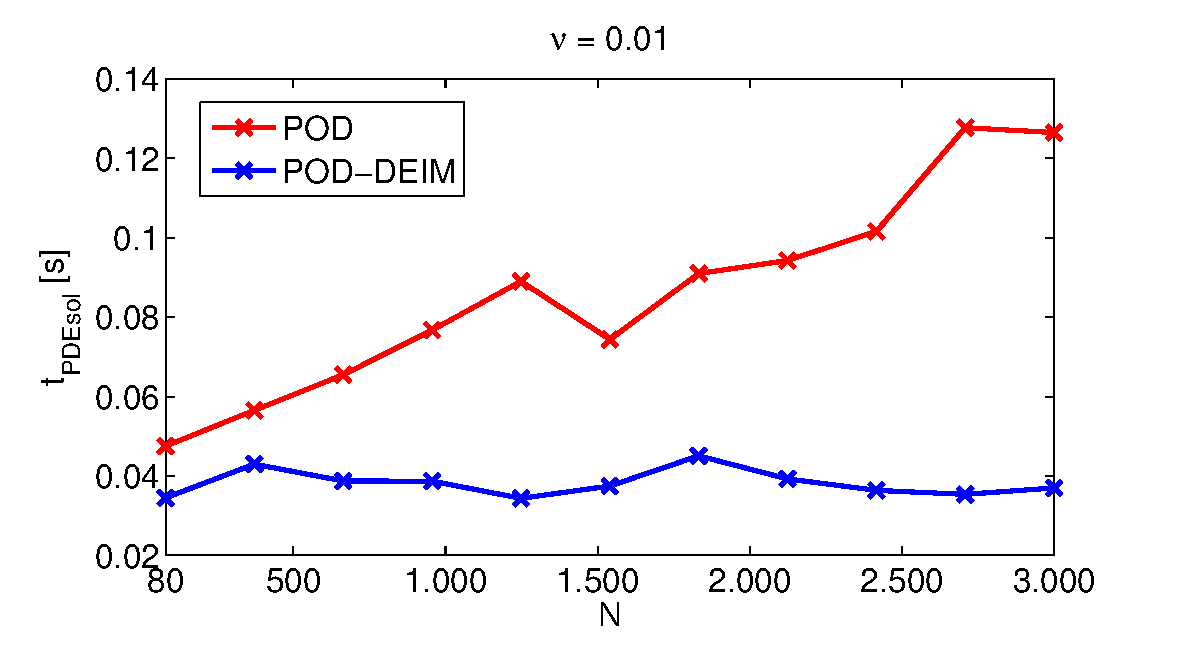
\includegraphics[width=0.49\textwidth]{figures/PODDEIM_Tsol}}
\end{figure}
}
\section[Optimal Control]{PDE-constrained optimization}
\frame{
\begin{block}{PDE-constrained optimization}
Minimize
\begin{align*}
\min_u \mathcal{J}(y(u),u),
\end{align*}
where $y$ is the solution to a nonlinear, possibly time-dependent partial differential equation,
\begin{align*}
c(y,u) = 0.
\end{align*}
\end{block}
\begin{itemize}
  \item $\mathcal{J}$ is called objective function,
  \item in order to evaluate $\mathcal{J}$, we need to solve $c(y,u)=0$ for $y(u)$,
  \item first-order and second-order optimization algorithms.
\end{itemize}
}
\subsection{A Newton-type method}
\frame{
\frametitle{A second-order optimization algorithm}
Minimize $\mathcal{J}(y(\cdot),\cdot)$ over $u$ taking information of the first and second derivative into account.\\
\hspace{0.2cm}
\begin{itemize}
  \item Choose $u_0$ and $k=0$
  \item Repeat until convergence
  \begin{itemize}
    \item[-] Solve the PDE-constraint $c(y_k,u_k)=0$ for $y_k$
    \item[-] Solve the Newton equation $\color{red} \nabla^2 \mathcal{J}(y_k,u_k) s_k = -\nabla \mathcal{J}(y_k,u_k)\color{black}$ via the \textbf{truncated CG-method}
    \item[-] Obtain $\alpha^* = \argmin_{\alpha \in \mathbb{R}_+} \mathcal{J}(y(u_k+\alpha s_k),u_k+\alpha s_k)$ via \textbf{Armijo line search}
    \item[-] Calculate new control $u_{k+1} = u_k + \alpha^* s_k$
    \item[-] Stop if $\|\nabla \mathcal{J}(y_k,u_k)\|$ is small or $\mathcal{J}(y_k,u_k)$ does not change anymore
    \item[-] $k = k + 1$
  \end{itemize}
\end{itemize}
}
\frame{
\frametitle{Gradient computation via adjoints}
Consider the Lagrangian function
\begin{align*}
\mathcal{L}(y,u,\lambda) = \mathcal{J}(y,u) + \lambda^T c(y,u)
\end{align*}
and \textbf{impose} the zero-gradient condition $\nabla_y \mathcal{L}(y,u,\lambda) = 0$.
\\ \vspace{0.2cm}
We derive the \textit{adjoint equation}:
\begin{align*}
\color{red} c_y(y(u),u)^T \lambda = -\nabla_y \mathcal{J}(y(u),u)\color{black}
\end{align*}
\setbeamercovered{transparent}
\uncover<2->{
\begin{algorithm}[H]
\small
\caption{\small{Computing $\nabla \mathcal{\hat J}(u)$ via adjoints \cite{H08}}}
\label{alg:Adj1}
\begin{algorithmic}[1]
\STATE For a given control $u$, solve $c(y,u) = 0$ for the state $y(u)$
\STATE Solve the adjoint equation $\color{red} c_y(y(u),u)^T \lambda = -\nabla_y \mathcal{J}(y(u),u)\color{black}$ for $\lambda(u)$
\STATE Compute $\nabla \mathcal{\hat J}(u) = \nabla_u \mathcal{J}(y(u),u) + c_u(y(u),u)^T \lambda(u)$
\end{algorithmic}
\end{algorithm}
}
}
\subsection{First-order methods: BFGS and SPG}
\frame{
\frametitle{First-order optimization algorithms}
\begin{itemize}
  \item Instead of solving $\nabla^2 \mathcal{J}(y_k,u_k) s_k = -\nabla \mathcal{J}(y_k,u_k)$, first-order methods \color{blue} approximate the Hessian \color{black} via $H_k$ and solve $H_k s_k = -\nabla \mathcal{J}(y_k,u_k)$,
  \item We have used \textsc{Matlab} implementations for the \color{blue} BFGS \color{black} and the \color{blue} SPG \color{black} method,
  \item Evaluation of $\mathcal{J}$ and gradient computation as seen before,
  \item \color{blue} SPG \color{black} easily allows to include bounds on the control, i.e. $u_{lower} \leq u(t,x) \leq u_{upper}$ which is used in many applications
\end{itemize}
}
\section[Burgers' equation]{Optimal Control for the reduced order Burgers' equation}
\subsection*{}
\frame{
\begin{block}{Optimal Control problem for Burgers' equation}
Minimize
\begin{align}
\label{minJ}
\min_{\color{red} u\color{black}} \frac{1}{2} \int_0^T \int_0^L [y(t,x) - \color{blue} z(t,x)\color{black}]^2 + \omega \color{red} u^2(t,x)\color{black} \ dx \ dt,
\end{align}
where $y$ is a solution to the nonlinear Burgers' equation
\begin{equation}
\label{Burgers2}
\begin{split}
y_t + \left( \frac{1}{2}y^2 - \nu y_x\right)_x = f + \color{red} u\color{black}&, \quad (x,t) \in (0,L) \times (0,T), \\
y(t,0) = y(t,L) = 0&, \quad t \in (0,T), \\
y(0,x) = y_0(x)&, \quad x \in (0,L).
\end{split}
\end{equation}
\end{block}
\begin{itemize}
  \item $\color{red} u \color{black}$ is the control that determines $y$
  \item $\color{blue} z \color{black}$ is the desired state
\end{itemize}
}
\frame{
\frametitle{Control goal}
We want to control the solution of Burgers' equation in such a way that it stays in the desired state $z(t,\cdot) = y_0, \forall t$:
\begin{figure}[H]
\centering
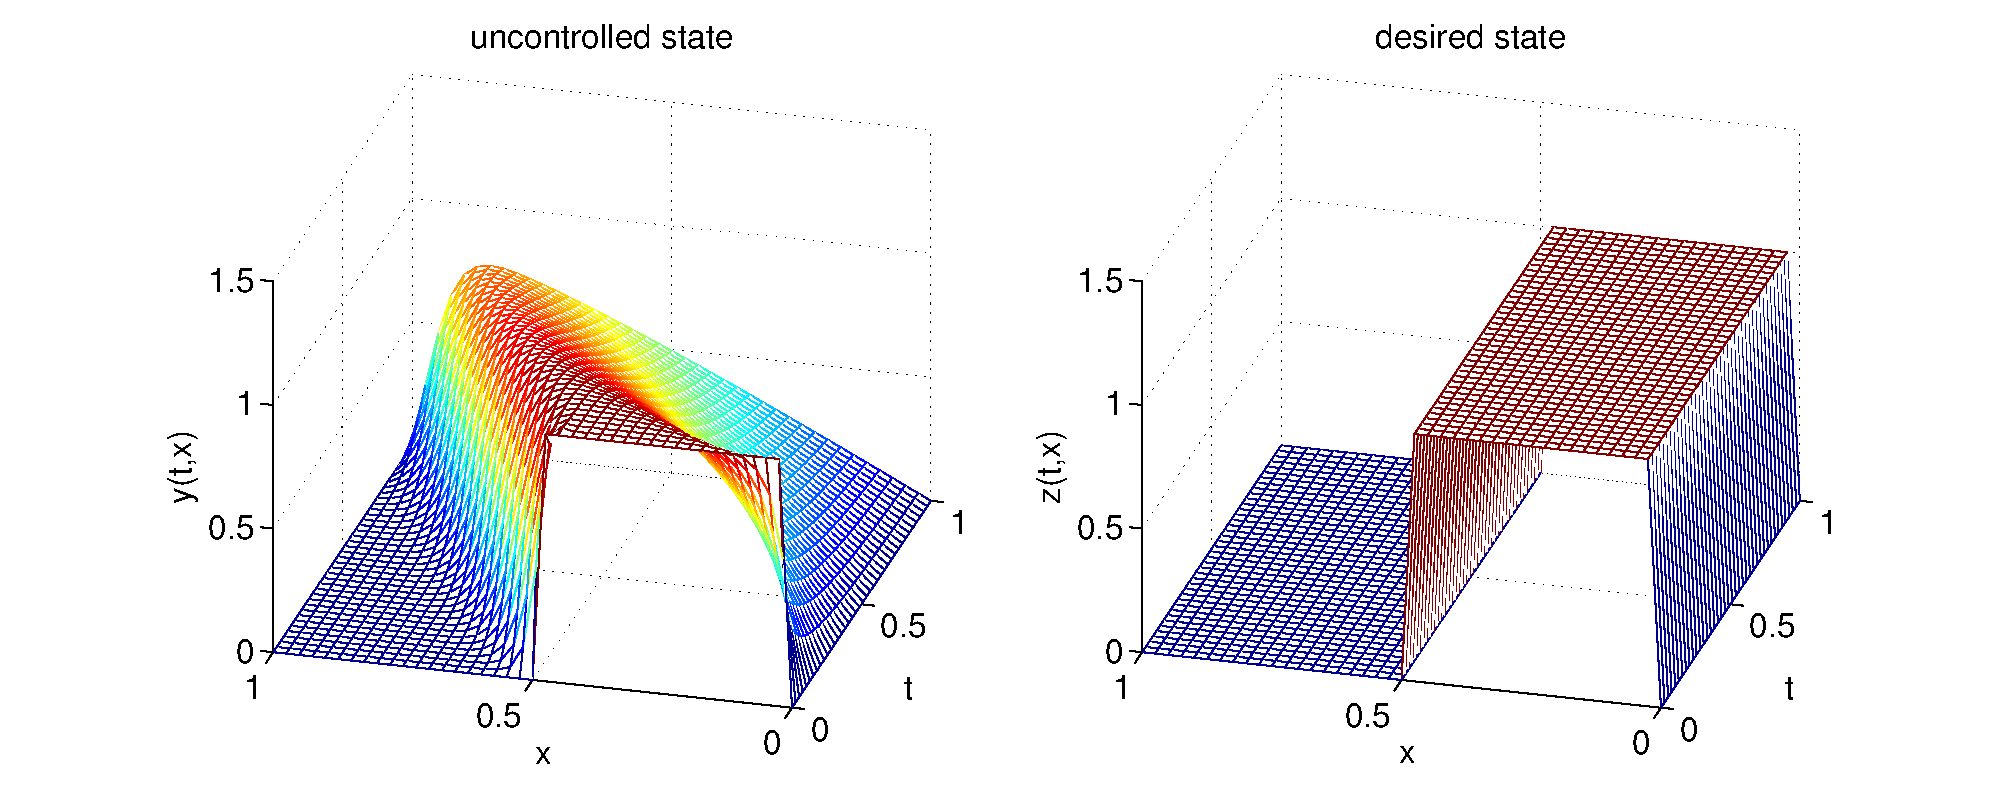
\includegraphics[width=0.9\textwidth]{../MSc/plots/desiredState}
\caption{Uncontrolled and desired state for $\nu = 0.01$.}\label{desState}
\end{figure}
}
%\subsection*{Discretization}
\frame{
\scriptsize{
\begin{block}{The full-order discretized optimal control problem}
\begin{align*}
 \min_u \mathcal{J}(y(u),u) \equiv \min_{\mathbf{u}_0,...,\mathbf{u}_{N_t}} \sum_{i=0}^{N_t} \delta \! t \left(\frac{1}{2}\mathbf{y}_i^T M \mathbf{y}_i - \mathbf{z}^T \mathbf{y}_i + \frac{\omega}{2} \mathbf{u}_i^T M \mathbf{u}_i  \right),
\end{align*}
where $\mathbf{y}_i$ is the solution of the full-order Burgers' equation
\begin{align*}
c(y,u) \equiv \frac{1}{\delta \! t} M \mathbf{y}_{i+1} - \frac{1}{\delta \! t} M \mathbf{y}_i + \frac{1}{2} B \mathbf{y}_{i+1}^2 + \nu C \mathbf{y}_{i+1} - \mathbf{f} - M \mathbf{u}_{i+1} = 0
\end{align*}
\end{block}
}
\scriptsize{
\begin{block}{The POD-DEIM reduced optimal control problem}
\begin{align*}
\min_u \mathcal{\tilde{J}}(\tilde{y}(u),u) \equiv \min_{\mathbf{u}_1,...,\mathbf{u}_{N_t}} \sum_{i=0}^{N_t} \delta \! t \left( \frac{1}{2} \mathbf{\tilde y}_i^T \mathbf{\tilde y}_i - \mathbf{\tilde z}^T\mathbf{\tilde y}_i + \frac{\omega}{2}\mathbf{u}_i^T M \mathbf{u}_i \right),
\end{align*}
where $\mathbf{\tilde y}_i$ is the solution of the POD-DEIM reduced Burgers' equation
\begin{align*}
\tilde{c}(\tilde{y},u) \equiv \frac{1}{\delta \! t} \mathbf{\tilde y}_{i+1} - \frac{1}{\delta \! t}\mathbf{\tilde y}_i + \frac{1}{2} \tilde{B}(\tilde{F}\mathbf{\tilde y}_{i+1})^2 + \nu \tilde{C}\mathbf{\tilde y}_{i+1} - \mathbf{\tilde f} - \tilde{M} \mathbf{u}_{i+1} = 0
\end{align*}
\end{block}
}
}
\frame{
\frametitle{Numerical tests}
Newton-type method for the full-order Burgers' model:
\begin{figure}[H]
\centering
\subfigure[$k=0$ (uncontrolled)]{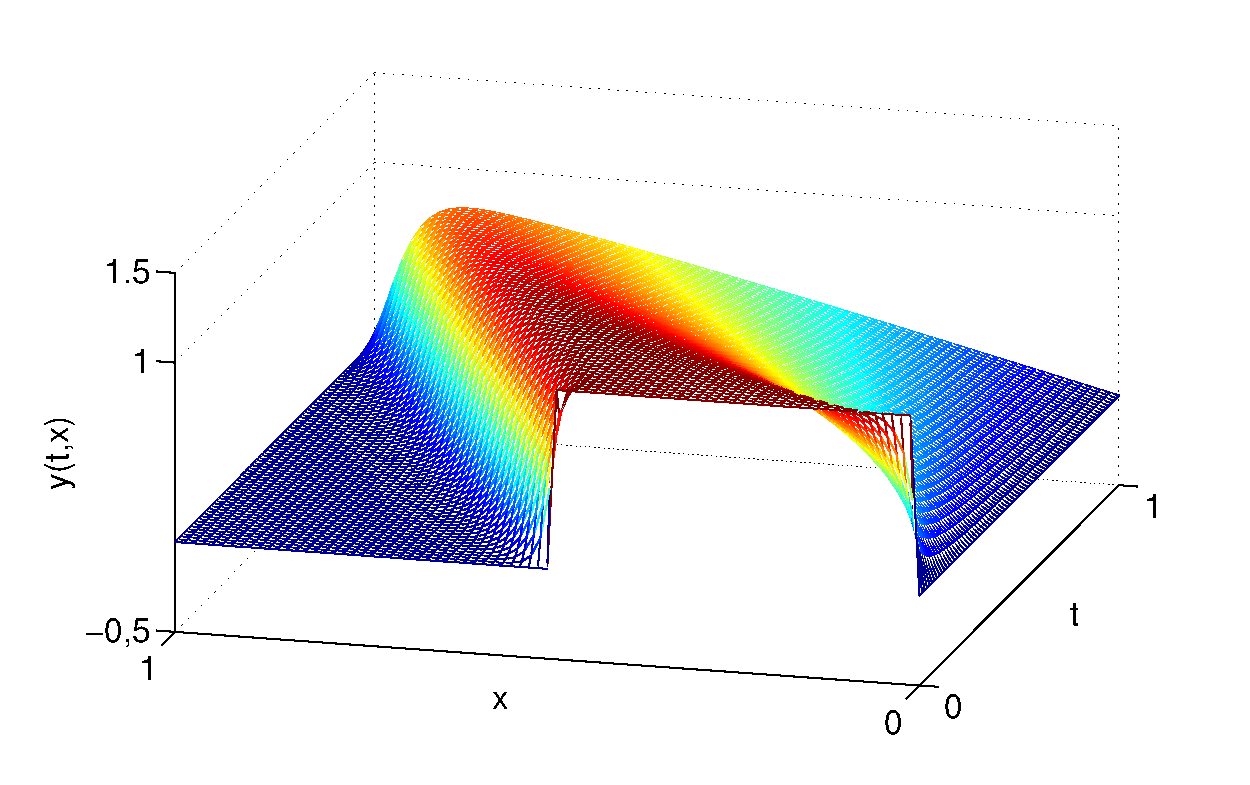
\includegraphics[width=0.33\textwidth]{../MSc/plots/controlFullk0_new}}\hfill
\subfigure[$k=1$ ]{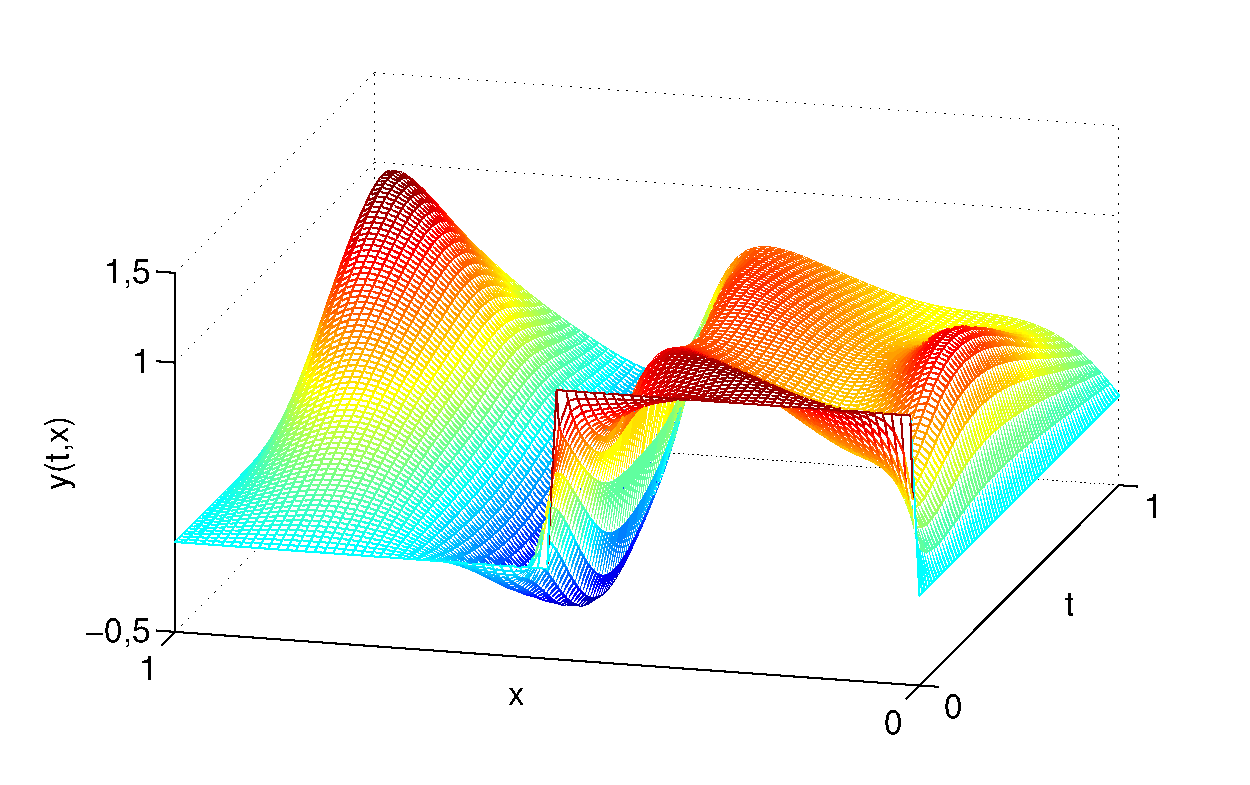
\includegraphics[width=0.33\textwidth]{../MSc/plots/controlFullk1_new}}\hfill
\subfigure[$k=2$]{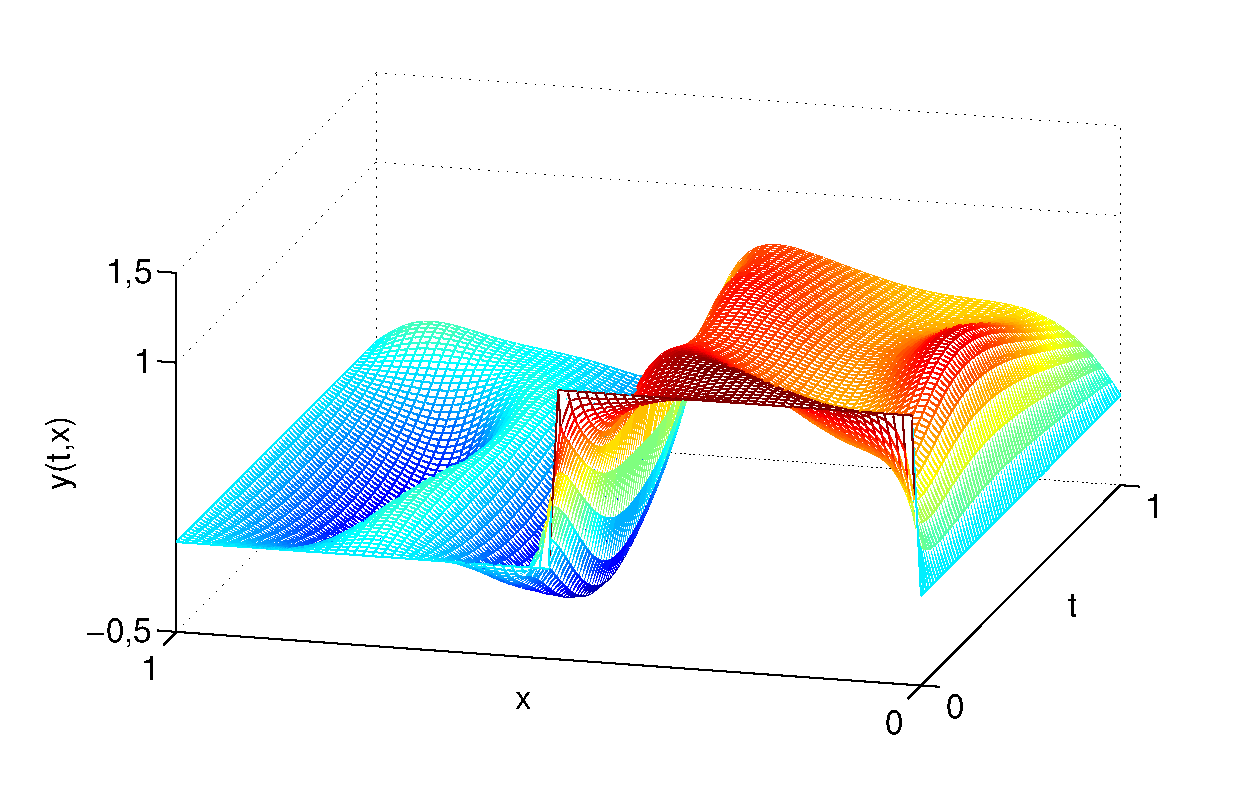
\includegraphics[width=0.33\textwidth]{../MSc/plots/controlFullk2_new}}\\
\subfigure[$k=3$ ]{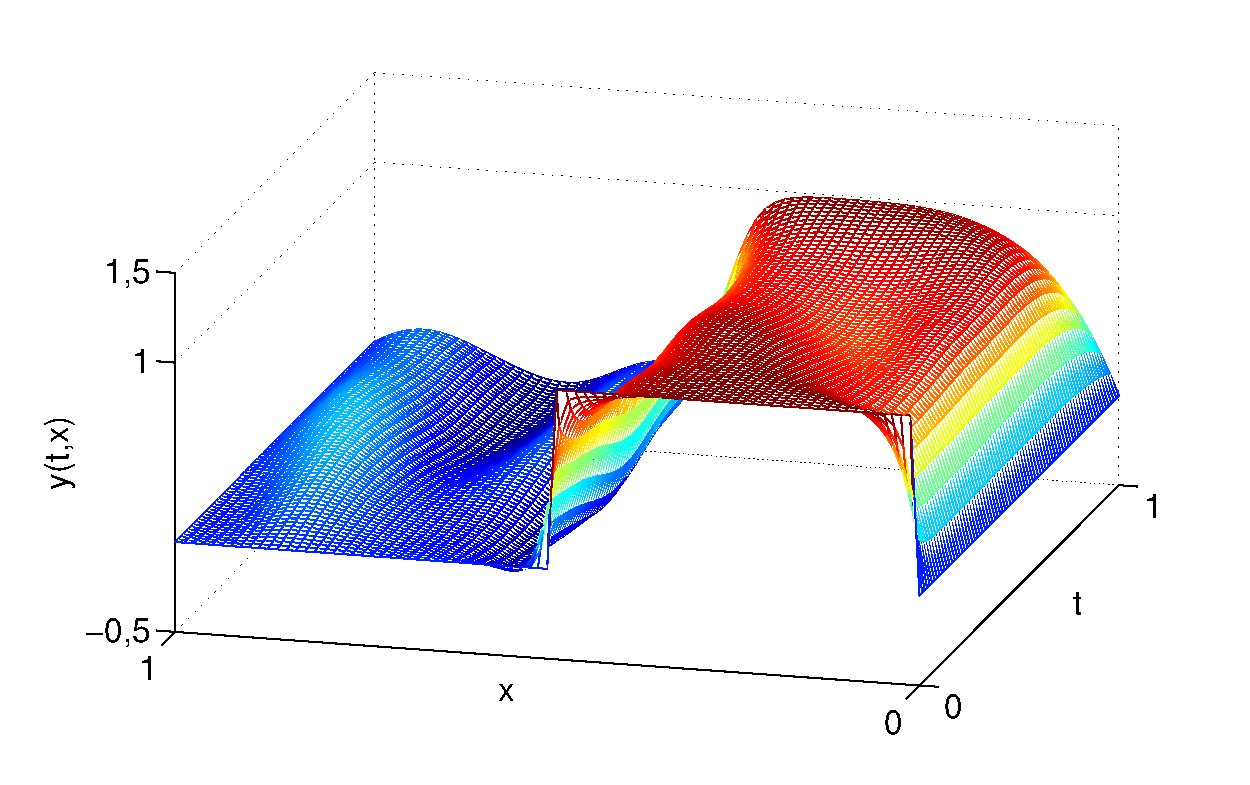
\includegraphics[width=0.33\textwidth]{../MSc/plots/controlFullk3_new}}\hfill
\subfigure[$k=4$ ]{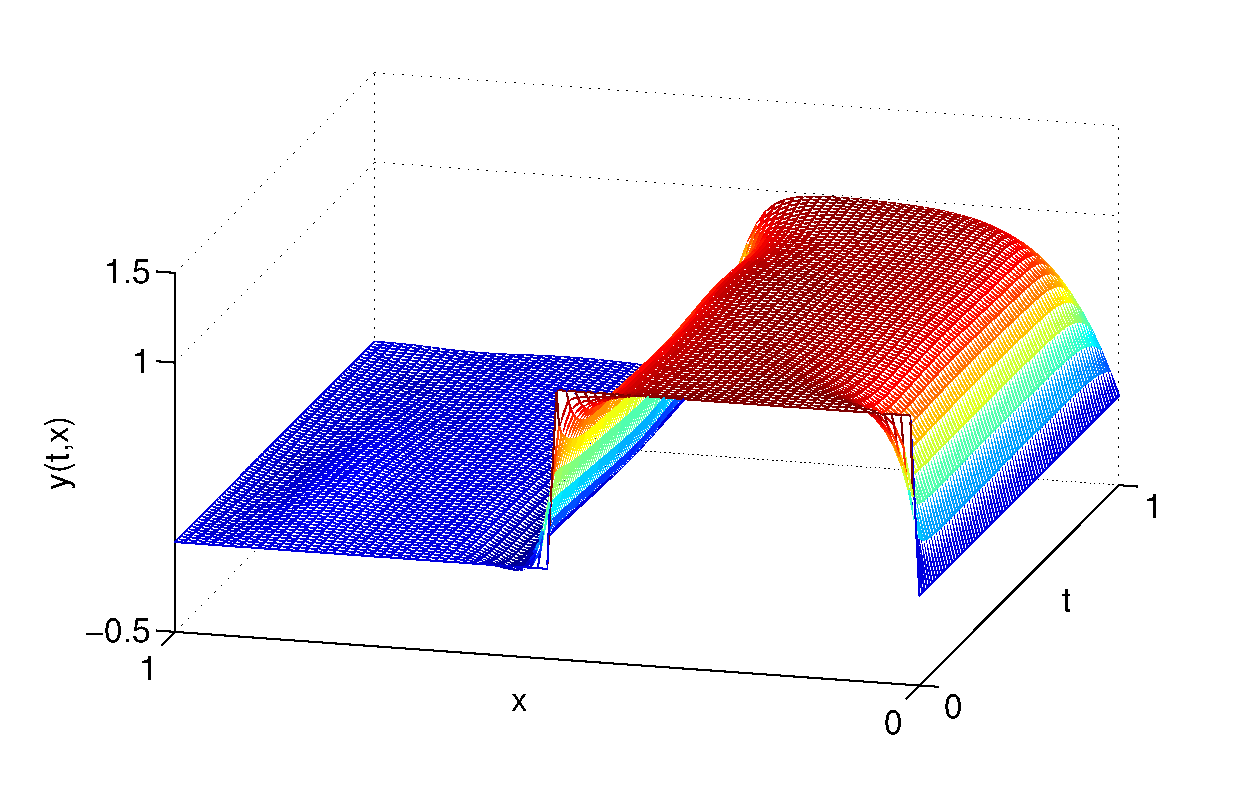
\includegraphics[width=0.33\textwidth]{../MSc/plots/controlFullk4_new}}\hfill
\subfigure[$k=5$]{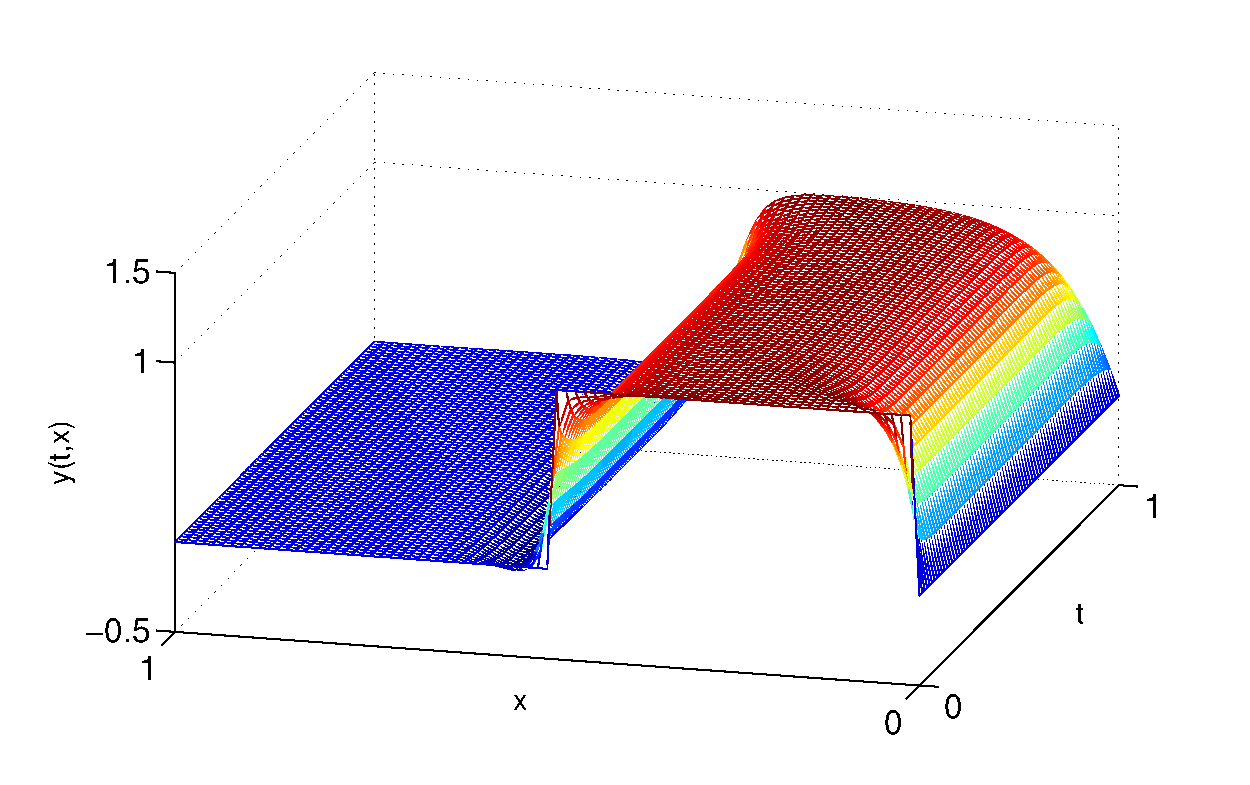
\includegraphics[width=0.33\textwidth]{../MSc/plots/controlFullk5_new}}\\
\end{figure}
}
\frame{
The corresponding optimal control at each iteration:
\begin{figure}[H]
\centering
\subfigure[$k=0$ (initial)]{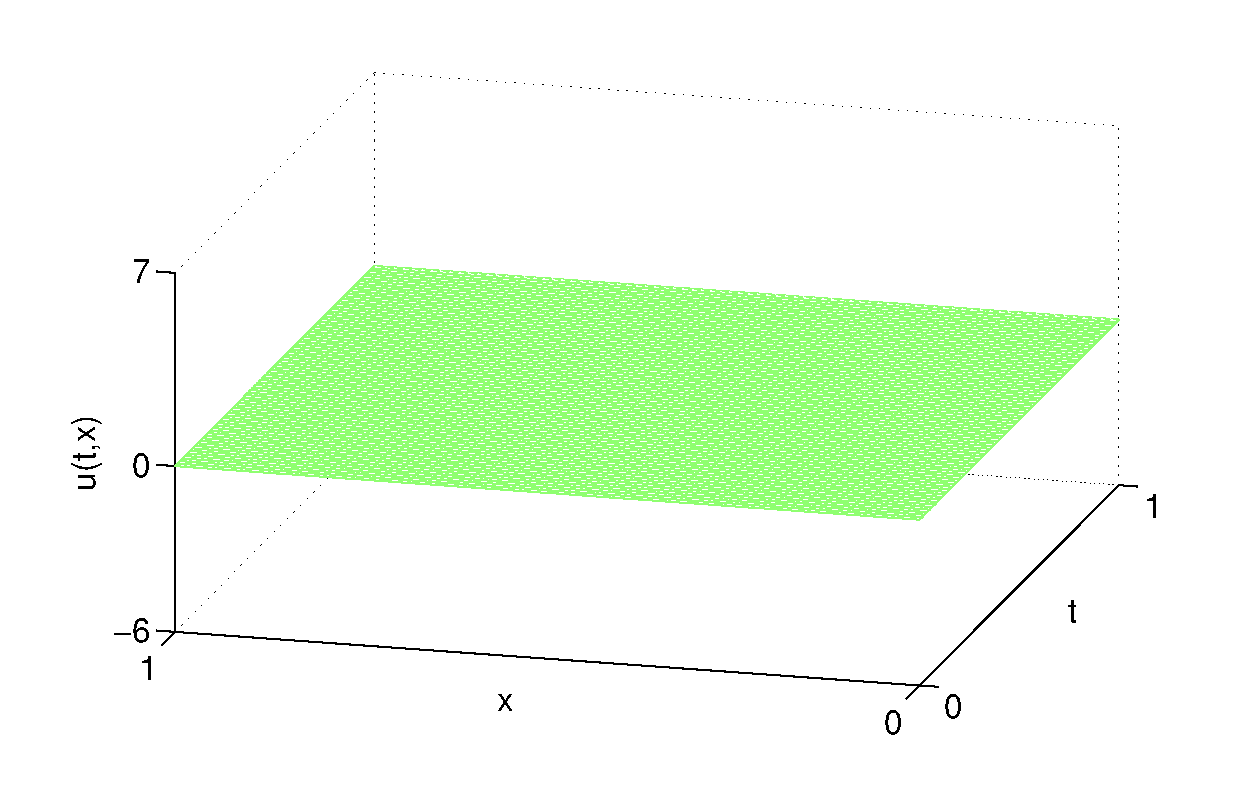
\includegraphics[width=0.33\textwidth]{../MSc/plots/uFullk0_new}}\hfill
\subfigure[$k=1$ ]{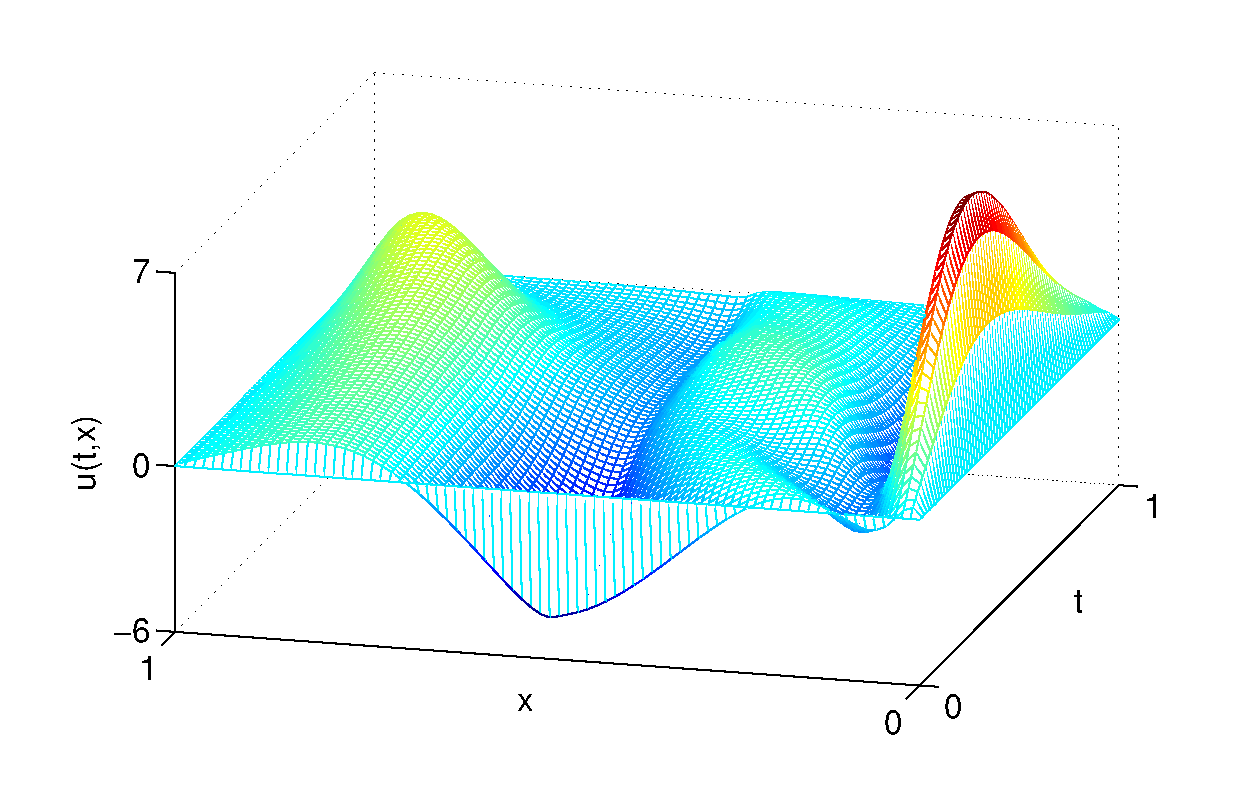
\includegraphics[width=0.33\textwidth]{../MSc/plots/uFullk1_new}}\hfill
\subfigure[$k=2$]{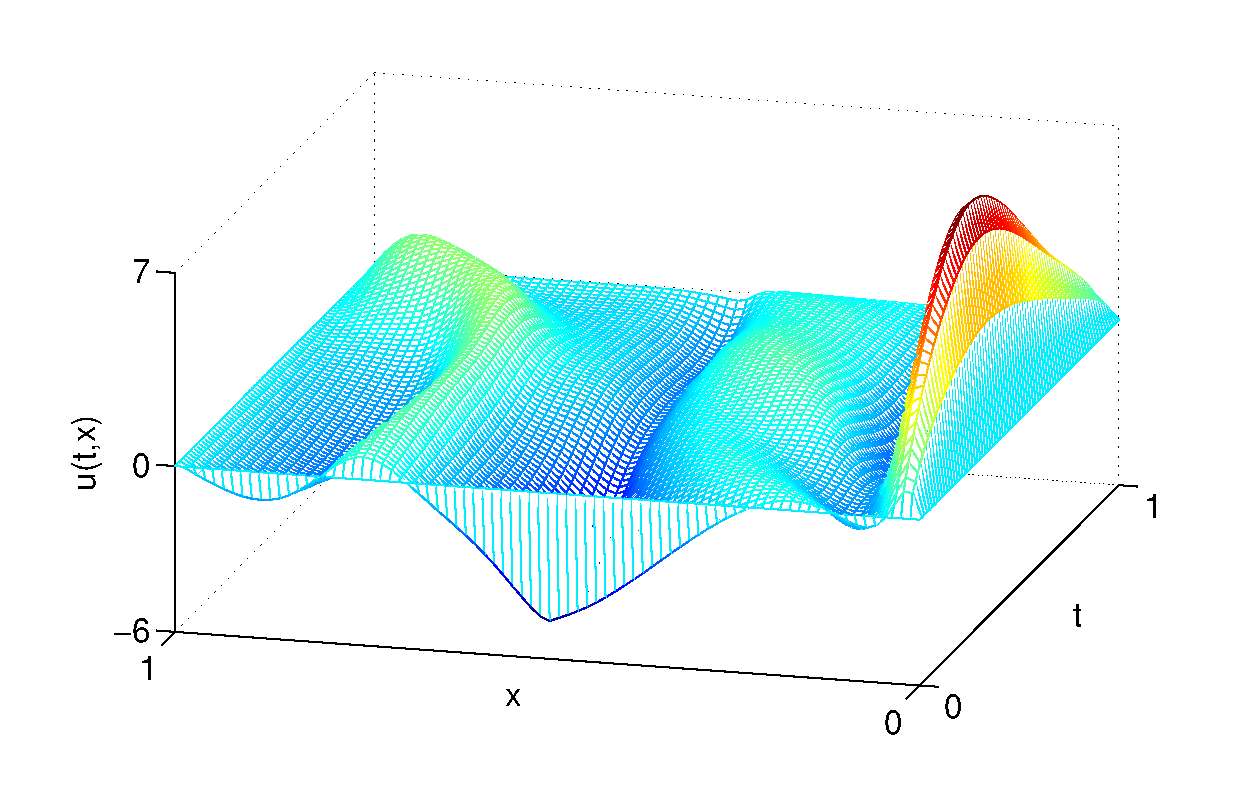
\includegraphics[width=0.33\textwidth]{../MSc/plots/uFullk2_new}}\\
\subfigure[$k=3$ ]{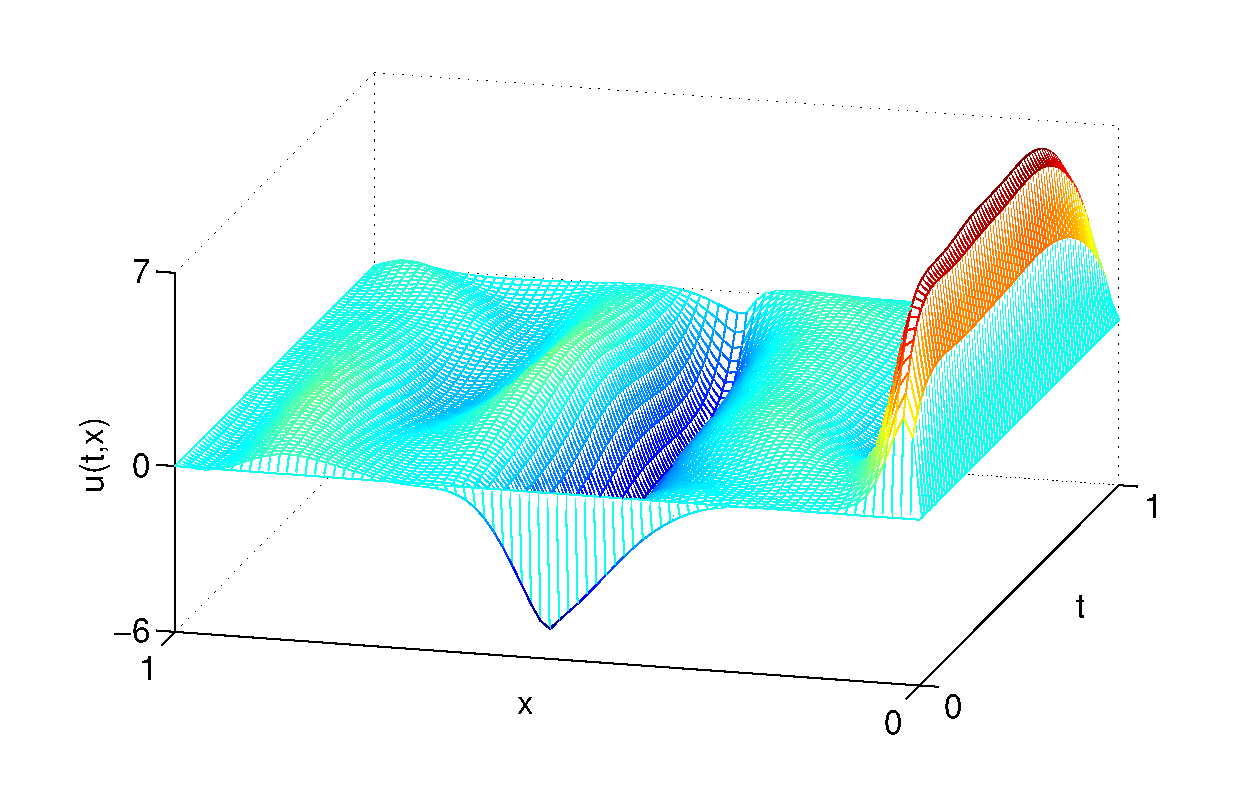
\includegraphics[width=0.33\textwidth]{../MSc/plots/uFullk3_new}}\hfill
\subfigure[$k=4$ ]{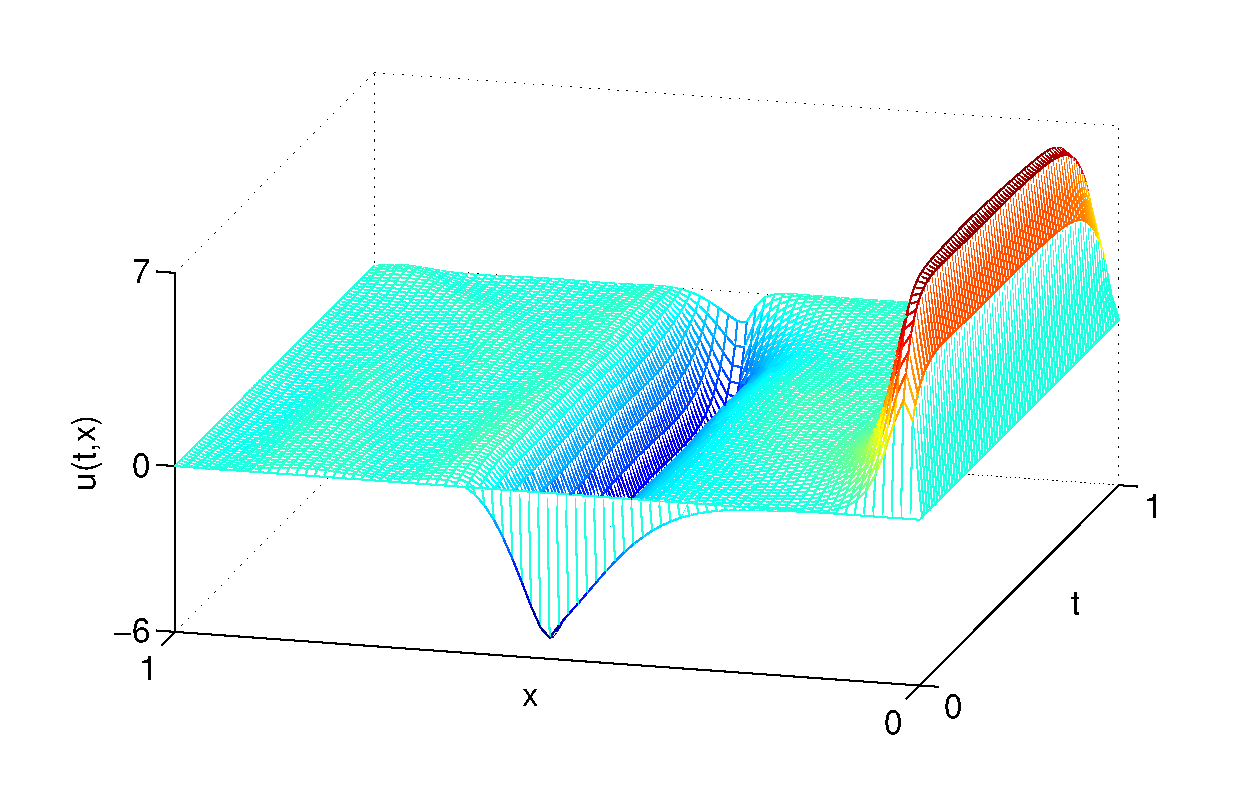
\includegraphics[width=0.33\textwidth]{../MSc/plots/uFullk4_new}}\hfill
\subfigure[$k=5$]{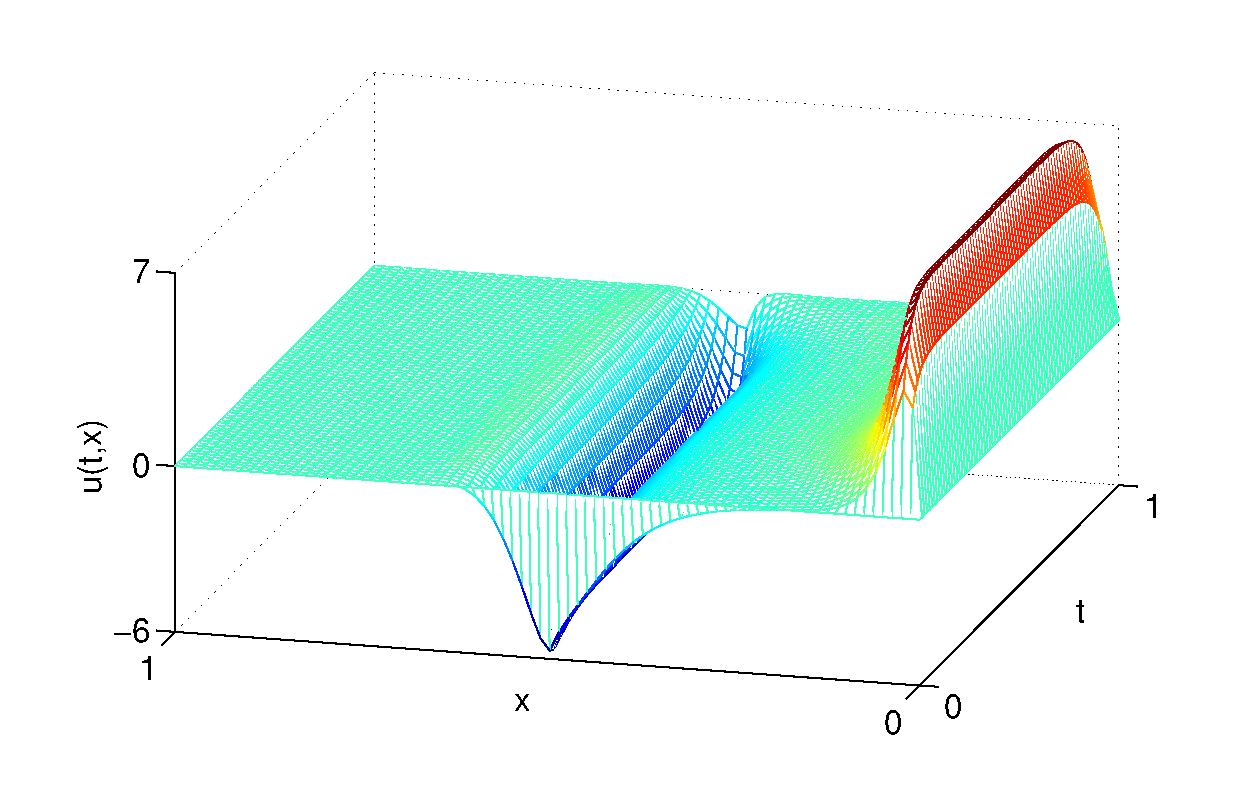
\includegraphics[width=0.33\textwidth]{../MSc/plots/uFullk5_new}\label{optFullu_opt}}\\
\end{figure}
}
\frame{
The following algorithm for \color{blue} POD-DEIM reduced optimal control \color{black} has been developed:\\
\hspace{0.2cm}
\begin{itemize}
  \item Choose $u^{(0)}$ for the full-order model, $K=0$
  \item Solve full-order Burgers' equation $c(y^{(0)},u^{(0)}) = 0$ for $y^{(0)}$
  \item Choose POD-dimension $\ell$ and DEIM-dimension $m$
  \item Repeat until $\|y^{(K)} - z\|_{L_2(\Omega)} < tol$
  \begin{itemize}
    \item[-] Perform POD-DEIM algorithm using snapshots of $y^{(K)}$ \\ $\quad \hookrightarrow \ \Phi_\ell, \mathcal{P}$
    \item[-] Solve $u^{(K+1)} = \argmin_u \mathcal{\tilde{J}}(\tilde{y}(u),u)$
    \item[-] Solve reduced Burgers' equation $\tilde{c}(\tilde{y}^{(K+1)},u^{(K+1)})=0$ for $\tilde{y}^{(K+1)}$
    \item[-] Expand $y^{(K+1)} = \Phi_\ell \tilde{y}^{(K+1)}$
    \item[-] $K = K + 1$
  \end{itemize}
\end{itemize}
}
\frame{
\begin{figure}[H]
\centering
\subfigure[$\ell = m = 7$]{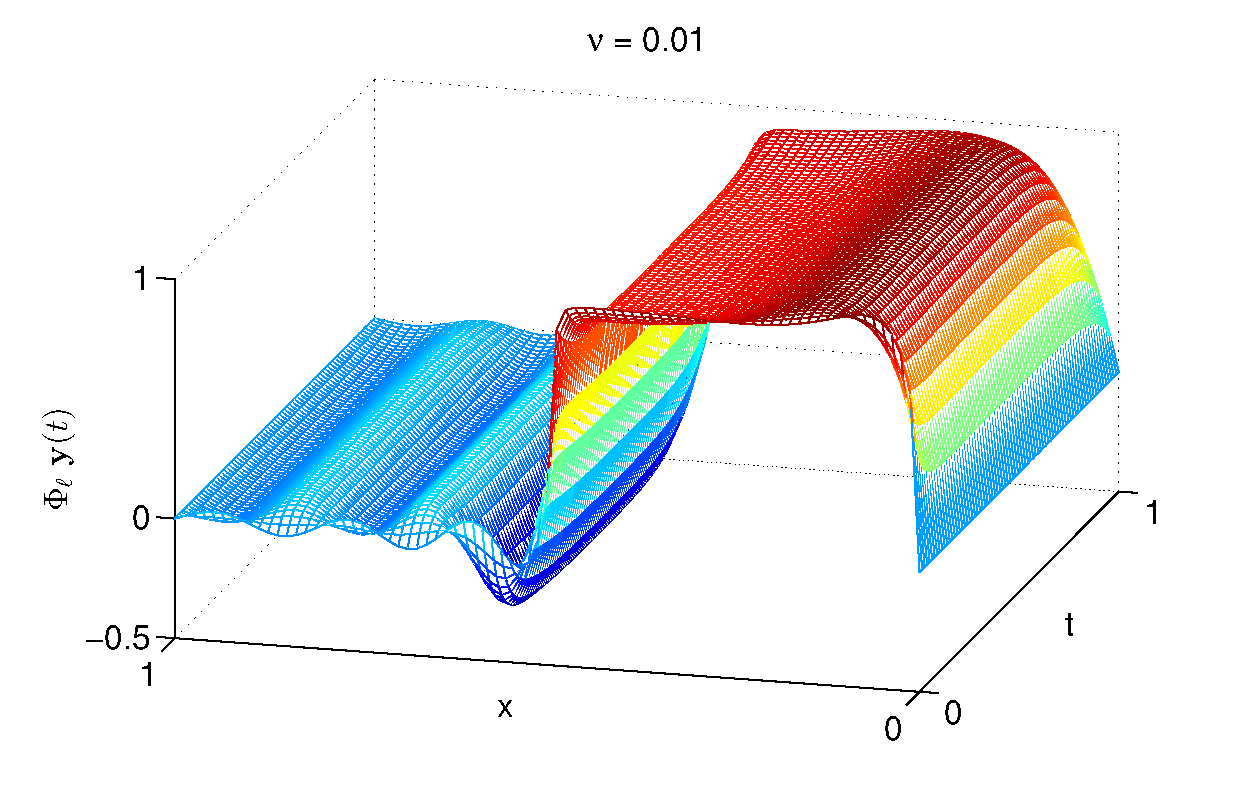
\includegraphics[width=0.4\textwidth]{../MSc/plots/redOptCon_y7}}
\subfigure[$\ell = m = 15$]{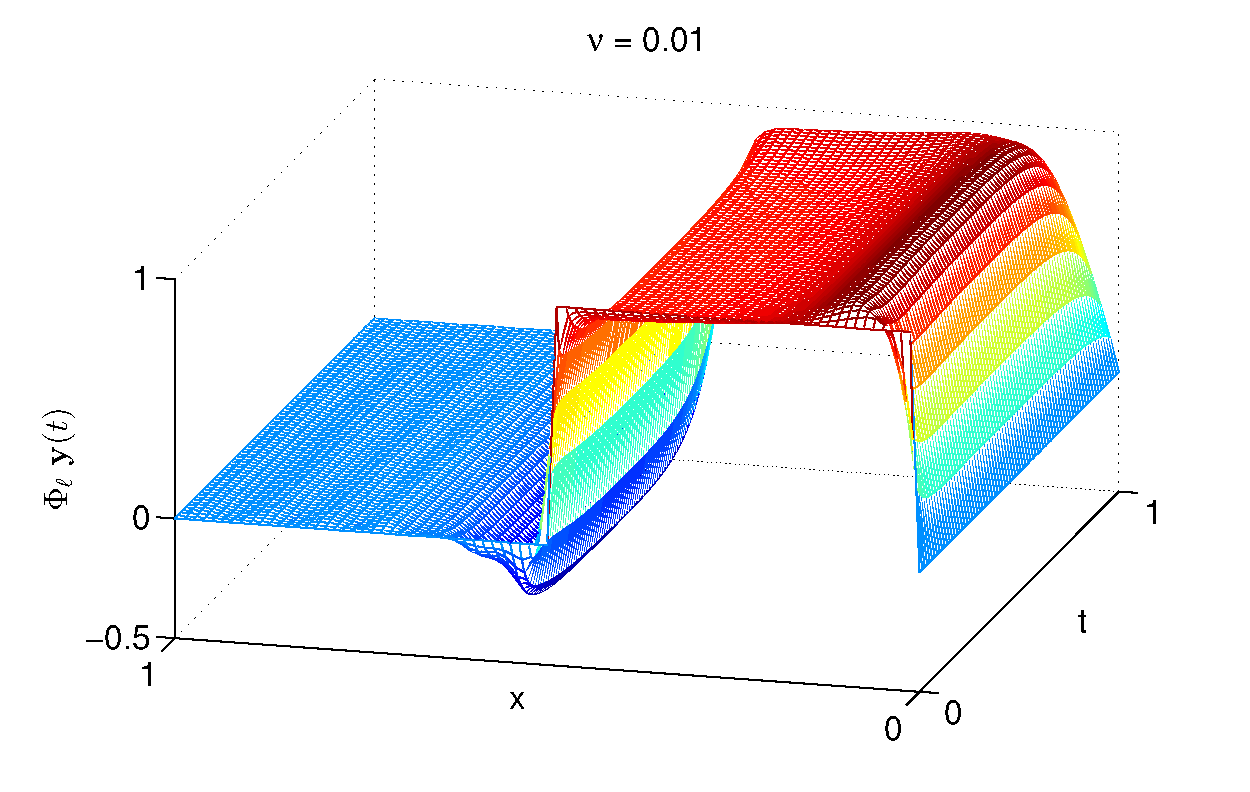
\includegraphics[width=0.4\textwidth]{../MSc/plots/redOptCon_y15}}\\
\subfigure[$\ell = m = 7$ ]{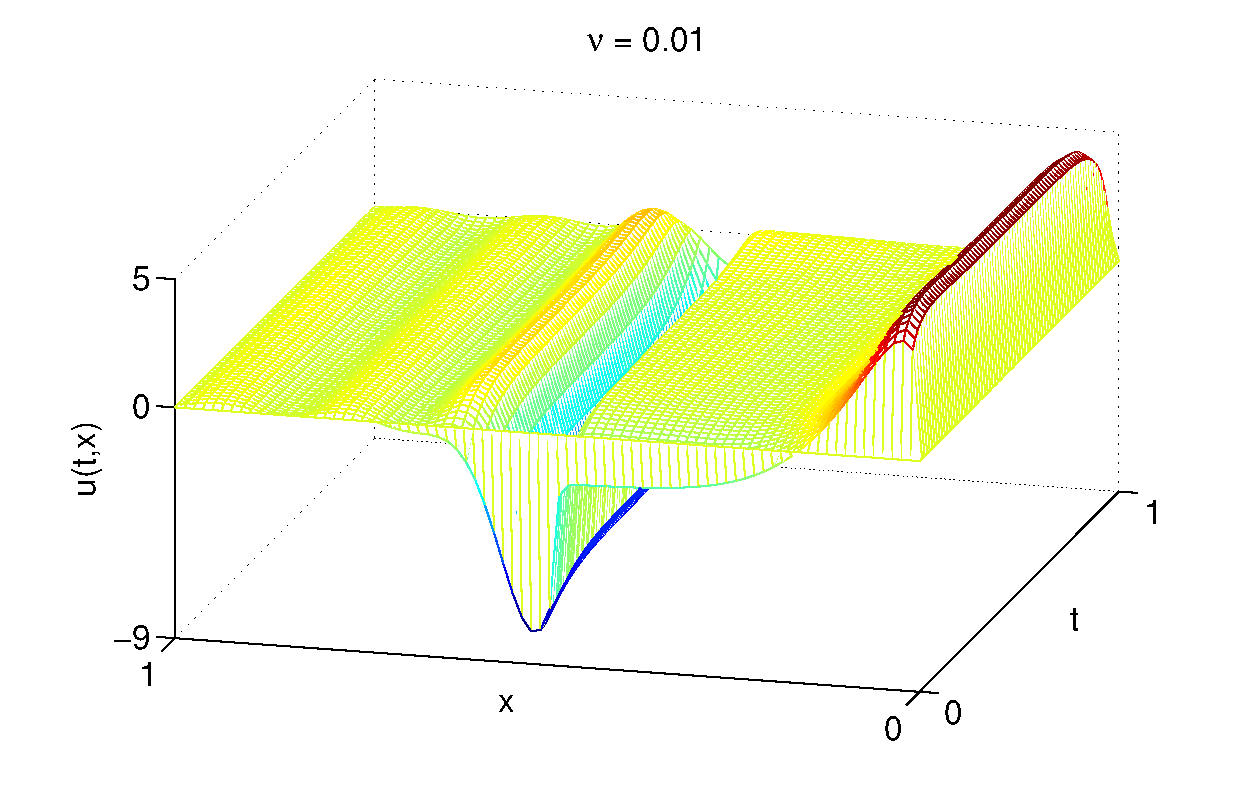
\includegraphics[width=0.4\textwidth]{../MSc/plots/redOptCon_u7}}
\subfigure[$\ell = m = 15$]{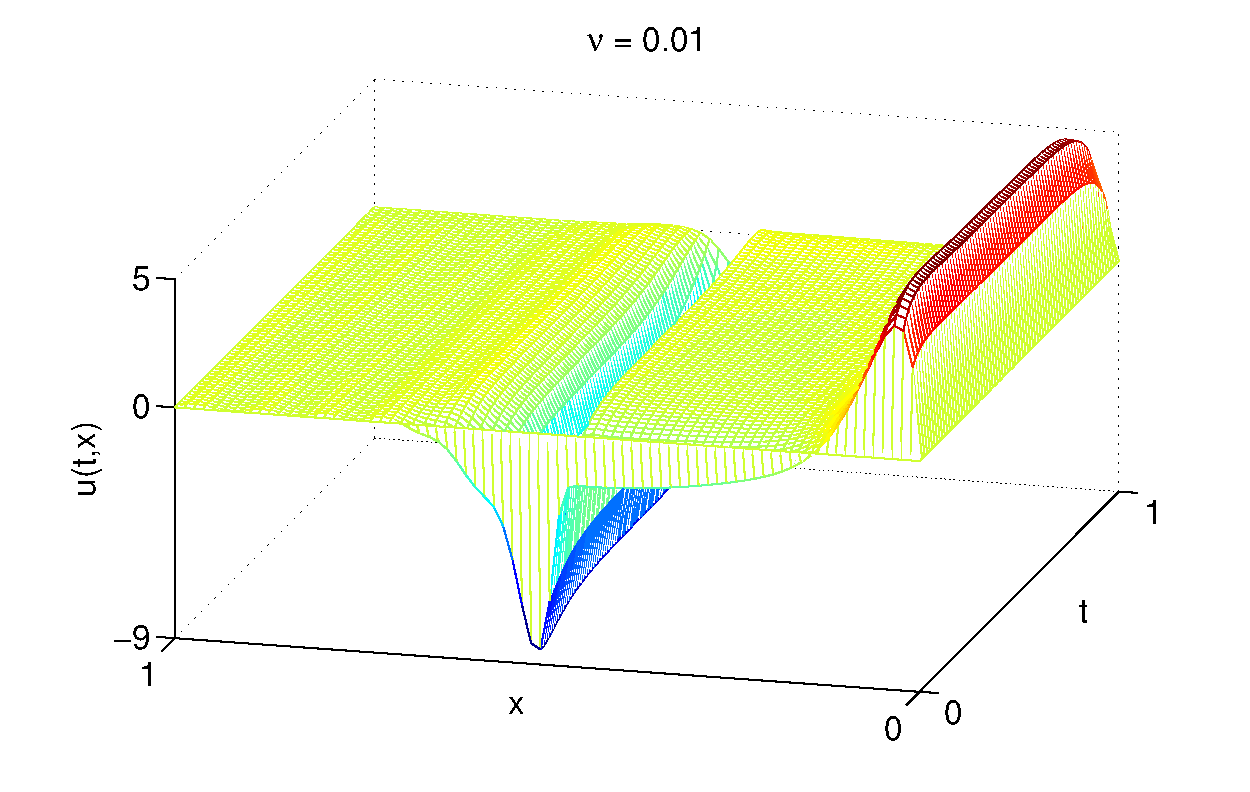
\includegraphics[width=0.4\textwidth]{../MSc/plots/redOptCon_u15}}\\
\end{figure}
}
\frame{
\frametitle{Computational benefit of the reduced optimization}
Newton-type optimization for different values of $\nu$:
\begin{figure}[H]
\centering
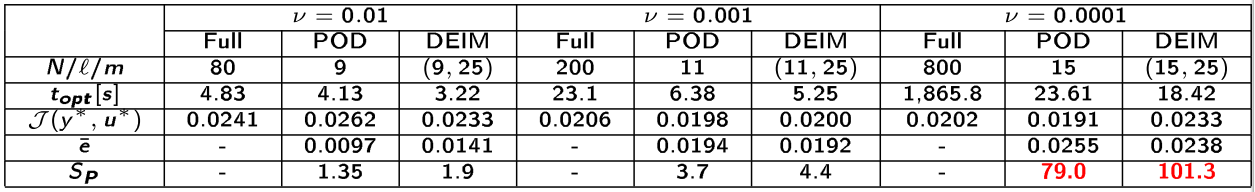
\includegraphics[width=1.\textwidth]{figures/longTabl.png}
\end{figure}
\setbeamercovered{transparent}
\uncover<2->{
Further numerical tests have shown:
\begin{itemize}
  \item For $\nu = 0.0001$ and $n_c = 3$ discrete control points in $[0,L]$, a speedup of $\sim 20$ for \color{blue} all three optimization methods \color{black} has been obtained.}
\uncover<3->{      
  \item For a bounded control $-2 \leq u(t,x) \leq 2$, optimization with \color{blue} SPG \color{black} leads to a speedup of $8.8$ using POD-DEIM and $\nu = 0.0001$.
\end{itemize}
}
%\begin{table}[H]
%\tiny
%\centering
%\begin{tabular}{|c|c|c|c|c|c|c|c|c|c|}
%\cline{1-10}
% & \multicolumn{3}{ c| }{$\nu = 0.01$} & \multicolumn{3}{ c| }{$\nu = 0.001$}& \multicolumn{3}{ c| }{$\nu = 0.0001$}\\ \cline{2-10}
% & Full & POD & DEIM & Full & POD & DEIM & Full & POD & DEIM \\ \cline{1-10}
%$N$/$\ell$/$m$ & $80$ &$ 9 $&$(9,25)$ &$200$ &$11$ &$(11,25)$ & $800$&$15$ & $(15,25)$\\ \cline{1-10}
%$t_{opt}[s]$        & 4.83      &4.13      &3.22       & 23.1 & 6.38 & 5.25 & 1,865.8 & 23.61 & 18.42 \\ \cline{1-10}
%$\mathcal{J}(y^*,u^*)$   &  0.0241      & 0.0262      &0.0233        & 0.0206 & 0.0198 & 0.0200 &0.0202 & 0.0191 &0.0233 \\ \cline{1-10}
%$\bar{e}$ &- & 0.0097 &  0.0141&- & 0.0194 & 0.0192 &- & 0.0255 &  0.0238\\ \cline{1-10}
%$S_P$           & -      &1.35       &1.9  & - &  3.7 & 4.4 & - & \color{red}\textbf{79.0}\color{black} &\color{red}\textbf{101.3}\color{black}\\ \cline{1-10}
%\end{tabular}
%\end{table}
}
\section[Outlook]{Summary and future research}
\subsection*{}
\frame{
\frametitle{Overview and main results}
\begin{itemize}
  \item Optimal Control of Burgers' equation using POD-DEIM leads to a \color{blue}speedup of $\sim 100$ \color{black} for small $\nu$.
  \item For the reduced model, all derivatives need to be computed in terms of the \color{blue}reduced variable\color{black}. This can be quite hard in practice.
  \item The \color{blue}accuracy \color{black} of the reduced Burgers' model is of the same order when POD is extended by DEIM.
\end{itemize}
}
\subsection*{}
\frame{
\frametitle{Future research questions}
\begin{itemize}
  \item Use the POD basis $\Phi_\ell$ also for \color{blue} dimension reduction of the control\color{black}, i.e.
   \begin{align*}
   \mathbf{u}(t) \approx \Phi_\ell \mathbf{\tilde u}(t) = \sum_{i=1}^\ell \varphi_i \tilde{u}_i(t)
   \end{align*}
  \item Extend Burgers' model to \color{blue} 2D/3D\color{black}
  \item More elaborated choice of reduced dimensions \color{blue} $\ell$ and $m$ \color{black}
\end{itemize}
}
\section*{}
\frame{
\begin{center}
This Master project is supervised by Marielba Rojas and \\ Martin van Gijzen.\\
\end{center}
\vspace{0.8cm}
\setbeamercovered{transparent}
\uncover<2->{
\begin{center}
\textbf{Thank you for your attention!}\\
\vspace{0.2cm}
Are there any questions or remarks?
\vspace{0.7cm}
\end{center}
\begin{center}
\url{https://github.com/ManuelMBaumann/MasterThesis}
\end{center}
}}
\section*{Literature}
\frame{
\frametitle{Further information can be found in...}
%\bibliographystyle{amsalpha}
%\bibliography{LitStudy.bib}
\begin{thebibliography}{10}
\small\setlength{\parskip}{0cm}
\bibitem[Chaturantabut, Sorensen, 2010]{DEIM}
S. Chaturantabut and D. Sorensen
\newblock {\em Nonlinear Model Reduction via Discrete Empirical Interpolation}.
\newblock SIAM Journal of Scientific Computing, 2010.
\bibitem[Heinkenschloss, 2008]{H08}
M. Heinkenschloss
\newblock {\em Numerical solution of implicitly constrained optimization problems}.
\newblock Technical report, Department of Computational and Applied Mathematics, Rice University, 2008.
\bibitem[Kunisch, Volkwein, 1999]{3}
K. Kunisch and S. Volkwein
\newblock {\em Control of the {B}urgers {E}quation by a {Reduced}-{Order} {A}pproach
	{U}sing {P}roper {O}rthogonal {D}ecomposition}.
\newblock Journal of Optimization Theory and Applications, 1999.
\end{thebibliography}
}
\end{document} 